\documentclass[Afour,sagev,times]{sagej}

\usepackage[T1]{fontenc}
\usepackage[utf8]{inputenc}
\usepackage{moreverb,url}
\usepackage{booktabs}
\usepackage{tabularx}
\usepackage{longtable}
\usepackage{array}
\usepackage{graphicx}
\usepackage{listings}
\usepackage{xcolor}
\usepackage{enumitem}
\usepackage{tikz}
\usetikzlibrary{shapes.geometric,arrows.meta,positioning,fit,backgrounds,calc}
\usepackage[colorlinks,bookmarksopen,bookmarksnumbered,citecolor=blue!50!black,urlcolor=blue!50!black,linkcolor=blue!50!black]{hyperref}

\newcommand{\code}[1]{\texttt{#1}}
\newcommand{\cq}[1]{\textsf{#1}}
\newcommand{\TODO}[1]{\textcolor{red}{\textbf{[TODO: #1]}}}

% Chowlk-style TikZ helpers
\tikzset{
  daimoclass/.style={rectangle, draw=black!70, fill=yellow!20, thick, rounded corners=2pt,
    minimum width=2.4cm, minimum height=0.7cm, align=center, font=\ttfamily\scriptsize,
    inner sep=3pt},
  externclass/.style={rectangle, draw=black!60, fill=blue!10, thick, rounded corners=2pt,
    minimum width=2.4cm, minimum height=0.7cm, align=center, font=\ttfamily\scriptsize,
    inner sep=3pt},
  modulebox/.style={rectangle, draw=black, fill=gray!15, thick,
    minimum width=3.0cm, minimum height=0.9cm, align=center, font=\sffamily\footnotesize\bfseries,
    inner sep=5pt},
  vocabbox/.style={rectangle, draw=black!60, fill=green!12, thick, rounded corners=3pt,
    minimum width=2.2cm, minimum height=0.65cm, align=center, font=\sffamily\scriptsize,
    inner sep=3pt},
  subclassarrow/.style={-{Triangle[open,length=2.5mm]}, draw=blue!70!black, thick},
  objpropertyarrow/.style={-{Latex[length=1.8mm]}, draw=black!80, thin},
  modulearrow/.style={-{Latex[length=1.8mm]}, draw=black!60, thick, dashed},
}

\newcolumntype{L}[1]{>{\raggedright\arraybackslash}p{#1}}

\lstset{
  basicstyle=\ttfamily\footnotesize,
  breaklines=true,
  columns=fullflexible,
  showstringspaces=false,
  frame=single,
  framerule=0pt,
  backgroundcolor=\color{gray!10},
  captionpos=b,
  aboveskip=0.8em,
  belowskip=0.8em
}

\def\volumeyear{2026}

\begin{document}

\runninghead{Mori Orrillo and Liu}

\title{DAIMO: an integration profile for AI-model governance across dataspaces}

\author{Edmundo de Elvira Mori Orrillo\affilnum{1} and Jiayun Liu\affilnum{1}}

\affiliation{\affilnum{1}Department of Artificial Intelligence, ETSI Inform\'aticos, Universidad Polit\'ecnica de Madrid, Spain}

\corrauth{Edmundo de Elvira Mori Orrillo, Universidad Polit\'ecnica de Madrid, Campus de Montegancedo, 28660 Boadilla del Monte, Madrid, Spain.}

\email{edmundo.mori.orrillo@upm.es}

\begin{abstract}
AI models increasingly circulate between organisations as governed assets, yet publishing a model, selecting it under a usage policy, invoking it through a typed service, tracing each execution, and comparing it under reproducible conditions are five operational tasks that today live in five different vocabularies: MLDCAT-AP describes the model, DCAT publishes it, ODRL expresses the policy, PROV-O records provenance, and the Dataspace Protocol (DSP) negotiates the contractual exchange. No existing ontology connects the five into a single governance chain.

We present DAIMO (\emph{Data-space AI Model Ontology}), an OWL~2~DL integration profile developed under the Linked Open Terms (LOT) methodology. DAIMO reuses the five vocabularies through seven \code{rdfs:subClassOf} and six \code{rdfs:subPropertyOf} alignments, and adds nine top-level native classes plus five role subclasses to cover the bridge constructs that no reused vocabulary provides: the offering record, the execution authorisation, the model deployment, the derived artefact, the cross-participant provenance bundle, the I/O contract, the audit evidence, and the shared evaluation context.

DAIMO ships three complementary evidence mechanisms. Consistency reasoning over the union of core and alignments is complemented by an \emph{entailment-verification check} that tests every inferred superclass of every native class against a list of semantically forbidden ones. A SHACL layer combines nine structural shapes, three conformance shapes over reused classes, and six cross-class SHACL-SPARQL invariants; each invariant is paired with a crafted violating case, and the negative test bench fires all six. An illustrative multi-participant demonstrator instantiates the profile, exercises every native class, and supports twenty-three competency questions elicited during requirements specification. The artefact is distributed as a public package with ontology, SHACL layer, demonstrator graph, SPARQL queries, validation scripts, and WIDOCO documentation.
\end{abstract}

\keywords{AI model governance; dataspace; ontology alignment; SHACL validation; LOT methodology}

\maketitle

% =====================================================================
\section{Introduction}\label{sec:intro}

Regulation (EU)~2024/1689, the \emph{AI Act}, requires for high-risk AI systems technical documentation of the model, a record of each execution, traceability of training, and audit evidence sustained across the full lifecycle~\cite{aiact}. In parallel, the European dataspace initiative, materialised in Eclipse Dataspace Components (EDC)~\cite{edc} connectors and sectoral deployments such as INESData and Gaia-X, establishes a contractual exchange model between autonomous participants on top of the Dataspace Protocol (DSP)~\cite{dsp}. These two frameworks, taken together, place AI models in a new regime: they must be able to circulate between organisations as governed assets, with actionable metadata that sustain publishing, discovering, invoking, tracing, and comparing them coherently. Semantic-Web vocabularies cover each of these five tasks in isolation, and this article argues that integrating them into a single profile is both necessary and non-trivial.

MLDCAT-AP~3.0.0 (SEMIC, 2025)~\cite{mldcatap} extends DCAT towards machine learning. An AI model becomes a catalog asset with task, algorithm, runs, evaluations, risks, and compute resources as first-class metadata. DCAT~\cite{dcat2} supplies the catalog primitives (\code{Catalog}, \code{Dataset}, \code{Distribution}, \code{DataService}, \code{CatalogRecord}) that MLDCAT-AP rests on. ODRL~\cite{odrl22} provides a mature model for offers, permissions, prohibitions, and agreements, and is the natural substrate for the usage policies that govern invocation. PROV-O~\cite{provo} is the standard for provenance and attribution across entities, activities, and agents. DSP~\cite{dsp} specifies the contract-negotiation and transfer messages that EDC implements. Model cards~\cite{mitchell19}, factsheets~\cite{arnold19}, and datasheets~\cite{gebru21} complement these vocabularies with narrative descriptions of intended use, limitations, and training conditions.

Each vocabulary solves its part. The gaps between them are the problem. A model published as \code{it6:MachineLearningModel} carries no attached act of being offered across an organisational boundary. An \code{odrl:Offer} is not anchored to a concrete model inside a federated catalog. A DSP negotiation is asset-agnostic: it does not know that the exchange concerns an AI model whose metrics and evaluation contexts condition its use. A \code{prov:Bundle} does not, by itself, group activities that occurred under distinct administrative contexts around the same derived artefact. Publishing, discovering, invoking, tracing, and comparing AI models in a dataspace requires these gaps to be articulated coherently.

\emph{No reusable ontology currently links catalog publication metadata, access policies, invocation contracts, execution traces, audit evidence, and comparative evaluation for AI models circulating between participants of a dataspace, with axiomatic alignments verified against existing vocabularies and with executable, reproducible evidence of correctness.} Closing that distance demands two simultaneous principles: we must reuse what the mature vocabularies already solve, and we must add only the constructs that the articulation between them requires.

We present DAIMO (\emph{Data-space AI Model Ontology}) and contribute three elements, supported by a reproducible illustrative demonstrator.

The \textbf{first} is the integration profile itself: an OWL~2~DL ontology that reuses DCAT-AP, MLDCAT-AP~3.0.0, ODRL~2.2, PROV-O, and DSP through seven \code{rdfs:subClassOf} and six \code{rdfs:subPropertyOf} alignments rather than bare prefix declarations. On top of that reuse layer, DAIMO introduces fourteen native classes that cover the bridge constructs absent from the union of the reused vocabularies. Each native class is justified by a concrete gap and by at least one competency question it answers. The delta over MLDCAT-AP is deliberately narrow: DAIMO reuses the AI-asset plane directly and adds only the governance bridge between the catalog and the dataspace.

The \textbf{second} is an \emph{entailment-verification} mechanism over the OWL-RL closure that complements standard consistency reasoning. For each native class, the check enumerates the inferred superclasses and tests them against a list of semantically forbidden ones. This catches alignments that a DL reasoner accepts without contradiction yet introduces unintended typings under reasoning.

The \textbf{third} is a SHACL layer that bundles six cross-class SPARQL invariants with a negative test bench. Each invariant comes with a purpose-built violating case. Validation conforms on the positive graph and fires all six violations on the negative graph, showing that the constraints are discriminating and not merely satisfiable.

As supporting evidence, we instantiate the profile over an illustrative multi-participant scenario with five anonymised actors (a model provider, a municipal consumer, a scientific evaluator, a federated dataspace platform, and a compliance office). The demonstrator exercises every native class at least once and supports all twenty-three competency questions. It is a reproducibility artefact, not a deployed pilot.


% =====================================================================
\section{Background and related work}\label{sec:related}

DAIMO sits at the intersection of three threads of work that the literature typically treats in isolation: describing AI models (narrative and structured), governing resources and dataspaces, and executable ontology engineering in the \emph{Semantic Web Journal}. We review each thread in turn, identifying what it contributes to the catalog-dataspace bridge, where it leaves the bridge open, and how DAIMO positions itself against it. Table~\ref{tab:reuse-matrix}, inspired by the reuse matrix of RePlanIT~\cite{kurteva}, compares the first two threads against the five operational attributes that any profile for governed AI models must cover.

\subsection{Describing AI models}

Descriptions of AI artefacts appear at two levels of formality. \emph{Narrative} documentation---model cards~\cite{mitchell19}, factsheets~\cite{arnold19}, and datasheets for datasets~\cite{gebru21}---raised transparency standards by describing intended use, limitations, performance on benchmarks, and training conditions in natural language. These formats are valuable for human readers and qualitative accountability, but insufficient as a substrate for automated discovery, policy-based filtering, or evidence linking in machine-to-machine flows.

Structured \emph{ontologies} of the ML lifecycle cover the machine-consumable layer. EXPO~\cite{expo} offers a general ontology of scientific experiments that later work has built on. ML-Schema~\cite{mls} formalises machine-learning experiments as a reusable, lightweight schema. MEX~\cite{mex} provides an interchange vocabulary, and OntoDM~\cite{ontodm} together with DMOP~\cite{dmop} organise the data-mining domain. Souza et al.~\cite{souza19} and Schmidt et al.~\cite{schmidt21} extend the perspective towards provenance and FAIRness across the lifecycle. These ontologies offer a rigorous foundation but remain centred on the scientific experiment and the training process; none addresses the contractual dimension of exchange between autonomous participants.

The work closest to DAIMO is MLDCAT-AP~3.0.0~\cite{mldcatap} (SEMIC, 2025). MLDCAT-AP extends DCAT to describe AI models as subclasses of \code{dcat:Dataset} with rich metadata on policy, benchmarks, evaluation, execution, risk, and compute infrastructure. DAIMO reuses it directly: \code{it6:MachineLearningModel} is the model class, and \code{it6:Task}, \code{it6:Run}, \code{it6:Flow}, \code{it6:Evaluation}, and \code{it6:ComputerInfrastructure} respectively capture the target task, the concrete execution, the associated pipeline, the resulting measurement, and the compute environment. MLDCAT-AP is strong on the model side but agnostic to the dataspace in which the model circulates: it does not model the act of offering a model across an organisational boundary, nor governed deployment, authorisation anchored to an agreement, or cross-participant provenance aggregation. MLDCAT-AP covers the model; DAIMO covers the bridge between the model and the dataspace.

Table~\ref{tab:mldcatap-delta} makes the MLDCAT-AP relationship explicit. For each MLDCAT-AP class most likely to co-occur with DAIMO, it records whether DAIMO reuses the class directly, imposes an additional conformance shape on it, or complements it with a new bridge class that MLDCAT-AP does not cover. The pattern is consistent: on the AI-asset plane DAIMO reuses and does not redefine; on the catalog-dataspace bridge DAIMO adds without overriding.

\begin{table*}[t]
\small\sf\centering
\caption{Relationship between DAIMO and MLDCAT-AP~3.0.0, class by class. \emph{Reuse direct} means DAIMO uses the class unchanged. \emph{Conformance} means DAIMO imposes a SHACL shape requiring a subset of properties on the class. \emph{Complement} means DAIMO introduces a new native class that MLDCAT-AP does not cover.\label{tab:mldcatap-delta}}
\begin{tabular}{@{}p{3.6cm}p{2.4cm}p{8cm}@{}}
\toprule
\textbf{MLDCAT-AP class} & \textbf{DAIMO treatment} & \textbf{Notes} \\
\midrule
\code{it6:MachineLearningModel} & Reuse + conformance & Reused as the AI asset; \code{MachineLearningModelInDAIMOShape} adds mandatory policy, title, identifier. \\
\code{it6:Task} & Reuse direct & Target task of a model; used as is. \\
\code{it6:Run} & Reuse + conformance & \code{RunInDAIMOShape} requires flow, algorithm, agent, timestamp; \code{daimo:authorizedBy} links runs to authorisations. \\
\code{it6:Flow} & Reuse direct & Pipeline associated with a run. \\
\code{it6:Evaluation} & Reuse direct & Measurement result; aggregated into \code{CrossParticipantProvenanceRecord} via \code{daimo:records}. \\
\code{it6:EvaluationMeasure} & Reuse direct & Metric type and value. \\
\code{it6:Benchmark} & Reuse direct & Benchmark reference; cited from \code{SharedEvaluationContext}. \\
\code{it6:ComputerInfrastructure} & Reuse direct & Compute environment on which a deployment runs. \\
\code{it6:Hardware}, \code{it6:Library} & Reuse direct & Elements of the compute environment. \\
\code{it6:HarmRisk} & Reuse direct & Risk annotation on a model. \\
\code{it6:Modality} & Reuse direct & Input modality. \\
\code{it6:trainedOn}, \code{it6:testedOn} & Reuse direct & Training/test dataset links. \\
\midrule
\multicolumn{2}{@{}l}{\textbf{Bridge constructs absent from MLDCAT-AP and added by DAIMO}} & \\
\midrule
(no MLDCAT-AP analogue) & Complement & \code{daimo:AIAssetOffering} -- catalog record with attached ODRL policy, aligned to \code{dcat:CatalogRecord}. \\
(no MLDCAT-AP analogue) & Complement & \code{daimo:ExecutionAuthorization} -- ODRL agreement that authorises concrete \code{it6:Run}s. \\
(no MLDCAT-AP analogue) & Complement & \code{daimo:ModelDeployment} -- typed link between model and \code{dcat:DataService}. \\
(no MLDCAT-AP analogue) & Complement & \code{daimo:IOContract} -- I/O formats and authentication method. \\
(no MLDCAT-AP analogue) & Complement & \code{daimo:DerivedArtifact} -- governable output of an authorised run. \\
(no MLDCAT-AP analogue) & Complement & \code{daimo:AuditEvidence} -- integrity record with \code{spdx:Checksum}. \\
(no MLDCAT-AP analogue) & Complement & \code{daimo:CrossParticipantProvenanceRecord} -- PROV bundle aggregating activities across \code{edc:ParticipantContext}s. \\
(no MLDCAT-AP analogue) & Complement & \code{daimo:SharedEvaluationContext} -- reified comparability conditions. \\
(no MLDCAT-AP analogue) & Complement & \code{daimo:ParticipantRole} + 5 subclasses -- role in dataspace exchange. \\
\bottomrule
\end{tabular}
\end{table*}

\subsection{Governing resources and dataspaces}

Two threads of work provide the governance substrate that DAIMO composes on top of the model description. The first is the family of W3C \emph{governance vocabularies} for resources. DCAT~2~\cite{dcat2} provides the catalog primitives on which MLDCAT-AP and DAIMO rest. ODRL~2.2~\cite{odrl22} offers a consolidated model for permissions, prohibitions, obligations, offers (\code{odrl:Offer}), and binding agreements (\code{odrl:Agreement}); DAIMO uses it extensively for the policy attached to offerings and for the agreements that authorise concrete executions. PROV-O~\cite{provo} provides the provenance ontology over activities, entities, agents, bundles, and roles, and is the natural substrate for tracing individual executions and their cross-participant aggregation. Pandit and Esteves~\cite{pandit-esteves} show how ODRL combines with DPV for health-data scenarios; DAIMO transposes that pattern to the AI domain. These vocabularies are mature and widely adopted but domain-agnostic: none is specific to AI, and none is specific to dataspaces.

The second thread is the emerging set of \emph{dataspace standards} that describe the exchange itself. Franklin et al.~\cite{franklin05} framed \emph{dataspaces} as a response to persistent heterogeneity, and Otto et al.~\cite{otto19} and Cappiello et al.~\cite{cappiello22} turn data sovereignty, contracts, and controlled interoperability into explicit design assumptions. The Dataspace Protocol~\cite{dsp} is the W3C-CG specification that defines catalog, contract-negotiation, and transfer-process messages; Eclipse Dataspace Components~\cite{edc} is its reference implementation. One distinction deserves emphasis: EDC is a Java execution framework, not an ontology. The semantics that EDC implements come from DSP (protocol), ODRL (policies), and DCAT (catalog); only a handful of concepts are genuine EDC-specific extensions, and of those DAIMO explicitly references \code{edc:ParticipantContext} to anchor aggregated provenance to an administrative context. Work on federated ecosystems such as ConSolid~\cite{werbrouck24} further shows that the Semantic Web is evolving towards multi-actor scenarios where governance and interoperability must be designed jointly.

\subsection{Executable ontology engineering in SWJ}

Beyond the domain substrate, a third thread of recent work shapes how DAIMO should be evaluated. The \emph{Semantic Web Journal} has recently published a body of ontologies that share an explicit methodological commitment to executable validation and reproducibility. Kurteva et al.\ present RePlanIT~\cite{kurteva}, an ontology for digital product passports of ICT equipment, with SHACL and industry-expert usability evaluation. Palma et al.\ operationalise soil information at global scale in GloSIS~\cite{palma} through a modular profile aligned with SOSA/SSN and ISO 28258. Woods et al.\ connect ontology engineering with natural-language processing for industrial maintenance activities~\cite{woods}. Bareedu et al.\ derive SHACL validation rules from OPC UA industry standards~\cite{bareedu24}. Ferranti et al.\ formalise Wikidata property constraints through SHACL and SPARQL~\cite{ferranti}. Robaldo and Batsakis~\cite{robaldo} examine the interplay between SHACL validation and inference on the Time Ontology. Penteado et al.~\cite{penteado23} study methodologies for publishing linked open government data. Collectively, these works set the expectation that an operationally oriented ontology ships reproducible evidence of correctness, not merely an axiomatic description. DAIMO meets that expectation.

\begin{table*}[t]
\small\sf\centering
\caption{Reuse matrix: families of related work against the five operational attributes that a profile for governed AI models must cover. $\bullet$ = natively covered; $\circ$ = partially covered via extensions; --- = not covered.\label{tab:reuse-matrix}}
\begin{tabular}{@{}lccccc@{}}
\toprule
\textbf{Family / artefact} & \textbf{Publication} & \textbf{Policy} & \textbf{Invocation} & \textbf{Traceability} & \textbf{Evaluation} \\
\midrule
Model cards, factsheets, datasheets~\cite{mitchell19,arnold19,gebru21} & $\circ$ & --- & --- & --- & $\circ$ \\
ML-Schema, MEX, OntoDM, DMOP~\cite{mls,mex,ontodm,dmop} & --- & --- & --- & $\circ$ & $\bullet$ \\
MLDCAT-AP 3.0.0~\cite{mldcatap} & $\bullet$ & $\circ$ & --- & $\bullet$ & $\bullet$ \\
DCAT 2~\cite{dcat2} & $\bullet$ & --- & $\circ$ & --- & --- \\
ODRL 2.2~\cite{odrl22} & --- & $\bullet$ & --- & --- & --- \\
PROV-O~\cite{provo} & --- & --- & --- & $\bullet$ & $\circ$ \\
DSP / EDC~\cite{dsp,edc} & $\circ$ & $\circ$ & $\bullet$ & --- & --- \\
\midrule
\textbf{DAIMO} (this work) & $\bullet$ & $\bullet$ & $\bullet$ & $\bullet$ & $\bullet$ \\
\bottomrule
\end{tabular}
\end{table*}

% =====================================================================
\section{Methodology and requirements}\label{sec:method}

We adopted the Linked Open Terms (LOT) methodology~\cite{lot22} for two reasons. First, its industrial orientation: LOT prescribes a lightweight workflow with deliverables at each of its four phases (requirements specification, implementation, publication, and maintenance). Second, LOT treats reuse as a first-class phase rather than a by-product, which matches the reuse-by-default discipline the problem demands. The subsections below describe the executive scenario that drove requirements elicitation (§\ref{sec:scenario}), the competency questions and non-functional requirements that resulted (§\ref{sec:method-req}), and the three core design decisions that shaped the ontology (§\ref{sec:method-design}).

\subsection{Illustrative scenario}\label{sec:scenario}

Requirements were elicited from an illustrative scenario in which five anonymised actor types exchange a geospatial risk-prediction model across a federated dataspace: \emph{Provider~A} (research organisation publishing the model), \emph{Consumer~B} (municipal consumer invoking predictions), \emph{Platform~C} (operator of the federated dataspace), \emph{Evaluator~D} (scientific evaluator publishing comparative measurements), and \emph{Compliance~E} (governance body auditing the chain). The scenario synthesises the five operational tasks a catalog-dataspace bridge must support: publishing, discovering, invoking, tracing, and evaluating. Section~\ref{sec:eval-usecase} describes the instantiation in detail. The scenario is a reproducibility demonstrator rather than a deployed pilot; replacing it by a real pilot with documented partners, or by an instantiation over a public MLDCAT-AP catalog, is a coherent next step.

\subsection{Requirements specification}\label{sec:method-req}

We elicited requirements from three complementary sources: the illustrative scenario of §\ref{sec:scenario}, the public specification of MLDCAT-AP~3.0.0, and the public documentation of Eclipse Dataspace Components and the Dataspace Protocol. From these sources we formulated twenty-three competency questions, organised into five categories by actor and lifecycle stage. Category R (registration and publication, five questions) covers the provider's need to publish a model as a governed asset with identity, licence, policy, and invocation contract. Category D (discovery and selection, four questions) captures the questions a consumer asks to locate a suitable model by task, domain, policy, and quality threshold. Category E (execution and auditability, five questions) groups the questions that a platform operator and a governance actor ask in order to invoke services, trace executions, and reconstruct evidence. Category V (evaluation and reproducibility, five questions) contains the evaluator's questions about comparing results under homogeneous conditions. Finally, category G (governance bridge, four questions) covers the multi-actor questions whose answer requires exclusively DAIMO-native semantics and, as we argue in §\ref{sec:discussion}, cannot be answered with the reused vocabularies alone. Table~\ref{tab:actors} summarises the actor-category mapping; the full set of twenty-three questions in natural language appears in Appendix~\ref{app:cqs}.

\begin{table*}[t]
\small\sf\centering
\caption{Actors involved in the executive scenario and the competency-question categories derived from them.\label{tab:actors}}
\begin{tabular}{@{}p{3.5cm}p{2cm}p{7cm}p{2.5cm}@{}}
\toprule
\textbf{Actor} & \textbf{Category} & \textbf{Need} & \textbf{CQs} \\
\midrule
Model provider & R & Publish a model as a governed asset with identity, licence, policy, and invocation contract & \cq{CQ-R1}--\cq{CQ-R5} \\
Model consumer & D & Discover models by task, domain, policy, and quality threshold & \cq{CQ-D1}--\cq{CQ-D4} \\
Platform operator & E & Invoke services, trace executions, and reconstruct operational evidence & \cq{CQ-E1}--\cq{CQ-E5} \\
Evaluator & V & Compare results under a shared context and inspect reproducibility & \cq{CQ-V1}--\cq{CQ-V5} \\
Governance (multi-actor) & G & Bridge offer, deployment, authorisation, and cross-participant provenance & \cq{CQ-G1}--\cq{CQ-G4} \\
\bottomrule
\end{tabular}
\end{table*}

Eleven of the twenty-three questions require explicit reasoning (subclass paths, subproperty chains, or SPARQL aggregation); the remaining twelve are direct queries over DAIMO-native data. This proportion is deliberate. A profile resting exclusively on direct queries would not exercise the part of the artefact that makes OWL semantics valuable, and a profile demanding reasoning for every question would be impractical on real endpoints.

Non-functional requirements fix the engineering constraints. The ontology targets the OWL~2~DL profile for decidability and HermiT compatibility, ships under CC-BY~4.0 (Apache~2.0 for the validation scripts), and uses persistent URIs under \url{https://w3id.org/pionera/daimo} with content negotiation and accessible SHACL validation. A reuse-by-default rule binds the modelling work: every DAIMO term must justify why none of DCAT, DCAT-AP, MLDCAT-AP, ODRL, PROV-O, DSP, or the EDC extension covers it.

\subsection{Core design decisions}\label{sec:method-design}

Three structural decisions shape the rest of the design.

\paragraph{Decision~1: reuse preferentially.} We reuse MLDCAT-AP classes directly whenever MLDCAT-AP already models the concept precisely. The model itself maps to \code{it6:MachineLearningModel}, the runtime environment to \code{it6:ComputerInfrastructure}, and the experimental triad of execution, pipeline, and measurement to \code{it6:Run}, \code{it6:Flow}, and \code{it6:Evaluation}. Publication and policy are similarly covered by existing vocabularies: \code{dcat:Dataset}, \code{dcat:Distribution}, and \code{dcat:DataService} on the DCAT side, \code{odrl:Offer} and \code{odrl:Agreement} on the ODRL side.

Introducing DAIMO-native equivalents for any of these would violate Gruber's principle of minimal ontological commitment and fracture the DCAT-AP ecosystem without adding expressive power. A native class is therefore justified only when the union of the reused vocabularies leaves a concrete gap that prevents answering at least one competency question.

\paragraph{Decision~2: separate three complementary planes.} The architecture distinguishes three planes that DAIMO connects but does not replace. Plane~A is the dataspace plane: DSP and the specific EDC extensions DAIMO references. Plane~B is the platform governance plane: INESData or an analogous platform, with its federated registration and operational policies. Plane~C is the AI/ML asset plane: MLDCAT-AP and the vocabularies that support it. DAIMO is the integration profile that connects A, B, and C; it is not a fourth parallel layer.

\paragraph{Decision~3: one native class per gap, not per theme.} Given reuse preference, each DAIMO-native class must justify its existence by a concrete gap in the union of the reused vocabularies and by at least one competency question that cannot be answered without it. Strict application of this criterion produces nine top-level classes (\code{AIAssetOffering}, \code{ParticipantRole}, \code{ModelDeployment}, \code{IOContract}, \code{ExecutionAuthorization}, \code{DerivedArtifact}, \code{CrossParticipantProvenanceRecord}, \code{AuditEvidence}, and \code{SharedEvaluationContext}) plus five role subclasses. Any candidate class failing both conditions simultaneously is discarded.

% =====================================================================
\section{The DAIMO ontology}\label{sec:ontology}

\subsection{Modular architecture and metrics}\label{sec:scope}

Five tasks define the scope: publication as a catalog record, policy-and-quality-sensitive discovery, invocation controlled by typed services, traceability of individual executions, and contextualised and reproducible evaluation. Orthogonal responsibilities (training-pipeline detail, fine-grained privacy-policy semantics, formal PROV derivation theory) already belong to mature vocabularies whose duplication would fracture the ecosystem. DAIMO adds the constructs that make those vocabularies articulate coherently when an AI model circulates between autonomous participants.

Three Turtle files decompose the ontology so that a consumer can load only what they need. The \textbf{core module} (\code{daimo-core.ttl}) contains the fourteen native classes, twenty-nine object properties and eight datatype properties, the global disjointness axioms, and the property characterisations (functional, asymmetric, inverse) that capture TBox-level type invariants. The \textbf{alignment module} (\code{alignment.ttl}) encapsulates the seven \code{rdfs:subClassOf} and six \code{rdfs:subPropertyOf} declarations that connect DAIMO to the reused vocabularies, plus minimal declarations of the external terms with \code{rdfs:seeAlso} pointers to their source specifications. The \textbf{SHACL module} (\code{daimo-shapes.ttl}) contributes eighteen \code{sh:NodeShape}s: nine structural, three of conformance over reused classes, and six cross-class invariants via \code{sh:SPARQLConstraint}. Because the module is declared as an independent \code{owl:Ontology} with its own \code{owl:versionIRI}, the validation layer has its own lifecycle.

\begin{figure}[t]
\centering
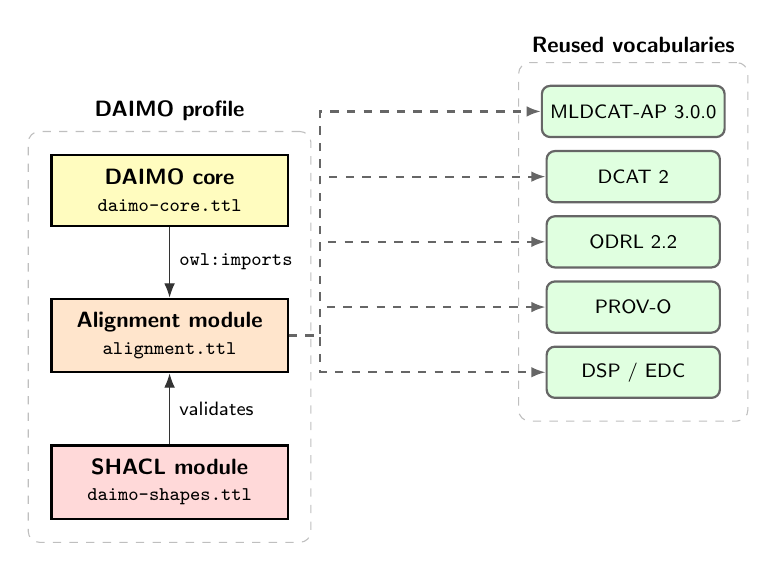
\begin{tikzpicture}[node distance=0.9cm and 0.7cm]
  % Three DAIMO modules (vertical stack on the left)
  \node[modulebox, fill=yellow!25] (core) {DAIMO core\\\scriptsize\normalfont\code{daimo-core.ttl}};
  \node[modulebox, fill=orange!20, below=of core] (align) {Alignment module\\\scriptsize\normalfont\code{alignment.ttl}};
  \node[modulebox, fill=red!15, below=of align] (shapes) {SHACL module\\\scriptsize\normalfont\code{daimo-shapes.ttl}};

  % Five reused vocabulary layers (vertical stack on the right)
  \node[vocabbox, right=3.2cm of core, yshift=1.0cm] (mldcat) {MLDCAT-AP 3.0.0};
  \node[vocabbox, below=0.15cm of mldcat] (dcat) {DCAT 2};
  \node[vocabbox, below=0.15cm of dcat] (odrl) {ODRL 2.2};
  \node[vocabbox, below=0.15cm of odrl] (prov) {PROV-O};
  \node[vocabbox, below=0.15cm of prov] (dsp) {DSP / EDC};

  % Arrows from alignment module (the bridge) to each vocabulary
  \draw[modulearrow] (align.east) -- ++(0.4,0) |- (mldcat.west);
  \draw[modulearrow] (align.east) -- ++(0.4,0) |- (dcat.west);
  \draw[modulearrow] (align.east) -- ++(0.4,0) |- (odrl.west);
  \draw[modulearrow] (align.east) -- ++(0.4,0) |- (prov.west);
  \draw[modulearrow] (align.east) -- ++(0.4,0) |- (dsp.west);

  % Core imports alignment (used by consumers who want inference)
  \draw[objpropertyarrow] (core.south) -- node[right, font=\scriptsize\sffamily] {\code{owl:imports}} (align.north);
  \draw[objpropertyarrow] (shapes.north) -- node[right, font=\scriptsize\sffamily] {validates} (align.south);

  % Legend
  \begin{scope}[on background layer]
    \node[fit=(core)(shapes), draw=gray!50, dashed, inner sep=8pt, rounded corners] (daimobox) {};
    \node[above=0.0cm of daimobox, font=\sffamily\footnotesize\bfseries] {DAIMO profile};
  \end{scope}
  \begin{scope}[on background layer]
    \node[fit=(mldcat)(dsp), draw=gray!50, dashed, inner sep=8pt, rounded corners] (vocbox) {};
    \node[above=0.0cm of vocbox, font=\sffamily\footnotesize\bfseries] {Reused vocabularies};
  \end{scope}
\end{tikzpicture}
\caption{Modular architecture of DAIMO and reused vocabularies. Yellow, orange, and red boxes denote the three DAIMO modules (core, alignment, shapes); green boxes denote the reused vocabularies. Dashed arrows from the alignment module carry the \code{rdfs:subClassOf} and \code{rdfs:subPropertyOf} declarations. The core module imports alignments for inference; the SHACL module validates data against the combined TBox.}
\label{fig:architecture}
\end{figure}

Table~\ref{tab:metrics} summarises the size and expressivity of the artefact, extracted directly from the Turtle files and from the reports produced by the validation suite (§\ref{sec:eval}). The numbers let a reader compare DAIMO with previously published ontologies in the same family.

\begin{table}[t]
\small\sf\centering
\caption{DAIMO artefact metrics verified against package files.\label{tab:metrics}}
\begin{tabular}{@{}p{4.6cm}r@{}}
\toprule
\textbf{Dimension} & \textbf{Value} \\
\midrule
Declared logical profile & OWL 2 DL \\
Native top-level classes & 9 \\
Native subclasses (\code{ParticipantRole}) & 5 \\
Total DAIMO-native classes & 14 \\
Object properties (\code{owl:ObjectProperty}) & 29 \\
Datatype properties (\code{owl:DatatypeProperty}) & 8 \\
Functional properties (\code{owl:FunctionalProperty}) & 28 \\
Asymmetric properties (\code{owl:AsymmetricProperty}) & 5 \\
Explicit inverse pairs (\code{owl:inverseOf}) & 5 \\
\code{rdfs:subClassOf} to externals & 7 \\
\code{rdfs:subPropertyOf} to externals & 6 \\
Named disjointness axiom & 1 \\
Total \code{sh:NodeShape}s & 18 \\
\quad completeness (one per DAIMO class) & 9 \\
\quad conformance over reused classes & 3 \\
\quad cross-class SPARQL invariants & 6 \\
Competency questions & 23 \\
OOPS! pitfalls (Critical/Important/Minor) & 0 / 0 / 2 \\
\bottomrule
\end{tabular}
\end{table}

\TODO{A complementary OntoMetrics-style table (Prot\'eg\'e plugin) is missing, breaking axiom counts down by type: SubClassOf, EquivalentClasses, DisjointClasses, ObjectPropertyDomain, ObjectPropertyRange, FunctionalObjectProperty, AsymmetricObjectProperty, InverseObjectProperties, SubDataPropertyOf, DataPropertyDomain, DataPropertyRange, AnnotationAssertion, etc. RePlanIT §5.2 and most SWJ ontology papers report this table; it gives the reviewer a quantitative measure of axiomatic richness independent of class and property counts.}

\subsection{Native classes and alignments}\label{sec:classes}

The nine top-level native classes, together with the five \code{ParticipantRole} subclasses, form the minimal set that the three core design decisions produce. Table~\ref{tab:classes} synthesises each class with its axiomatic alignment to the reused vocabularies; the subsections that follow examine those that carry the most semantic load. Figure~\ref{fig:classes} shows the overall view of classes and native properties.

\begin{table*}[t]
\small\sf\centering
\caption{DAIMO-native classes, axiomatic alignments, and the competency questions they answer.\label{tab:classes}}
\begin{tabular}{@{}p{4cm}p{3cm}p{6cm}p{2.2cm}@{}}
\toprule
\textbf{Class} & \textbf{Alignment} & \textbf{Role} & \textbf{CQs} \\
\midrule
\code{daimo:AIAssetOffering} & \code{dcat:CatalogRecord} & Catalog record that publishes a model as a governed offer in a dataspace; carries an ODRL policy via \code{daimo:hasOfferPolicy}. & R1, R2, R5, G1 \\
\code{daimo:ParticipantRole} \newline (+5 non-disjoint subclasses) & \code{prov:Role} & Role a participant plays with respect to an AI asset within a dataspace context. & R5 \\
\code{daimo:ModelDeployment} & \code{prov:Entity} & Running or hosted instance of a model, exposed as a \code{dcat:DataService} over an \code{it6:ComputerInfrastructure}. & E1, E3, G2 \\
\code{daimo:IOContract} & (no external alignment) & Minimal actionable contract: I/O formats, authentication method, optional schemas. & R4, E1, G2 \\
\code{daimo:ExecutionAuthorization} & \code{odrl:Agreement} & ODRL agreement derived from a DSP negotiation that authorises concrete executions via \code{daimo:authorizesRun}. & E2, E5, G3 \\
\code{daimo:DerivedArtifact} & \code{prov:Entity}, \code{dcat:Resource} & Governed and catalogable output produced by an execution under authorisation. & E5, G4 \\
\code{daimo:CrossParticipantProvenanceRecord} & \code{prov:Bundle} & Aggregation of activities and entities across participant contexts forming an audit narrative. & G4 \\
\code{daimo:AuditEvidence} & \code{prov:Entity} & Compliance-oriented evidence record with structured \code{spdx:Checksum}, signer, and timestamp. & E4 \\
\code{daimo:SharedEvaluationContext} & (no external alignment) & Reified comparability conditions: task, dataset, version, protocol, and random seed. & V1, V2, V3 \\
\bottomrule
\end{tabular}
\end{table*}

\begin{figure*}[t]
\centering
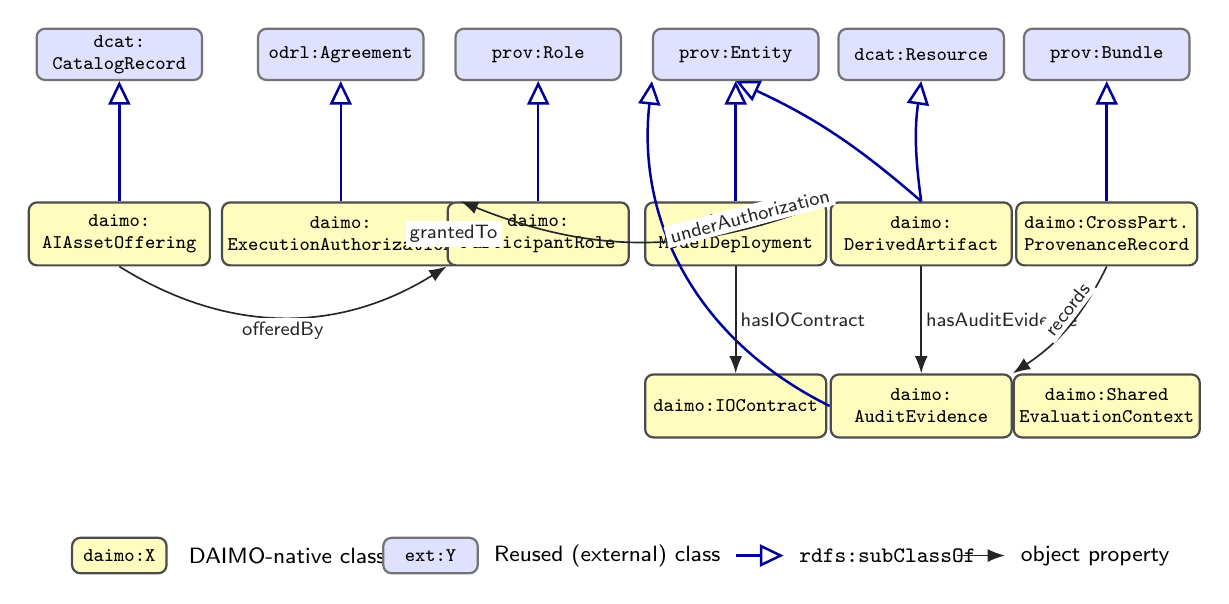
\begin{tikzpicture}[
    x=0.76cm, y=0.95cm,
    daimoclass/.style={rectangle, draw=black!70, fill=yellow!25, thick,
      rounded corners=3pt, minimum width=2.3cm, minimum height=0.8cm,
      align=center, font=\ttfamily\scriptsize, inner sep=2pt},
    externclass/.style={rectangle, draw=black!55, fill=blue!12, thick,
      rounded corners=3pt, minimum width=2.1cm, minimum height=0.65cm,
      align=center, font=\ttfamily\scriptsize, inner sep=2pt},
    subarrow/.style={-{Triangle[open,length=3mm,width=2.8mm]},
      draw=blue!60!black, line width=0.9pt},
    proparrow/.style={-{Latex[length=2.2mm]}, draw=black!85, line width=0.6pt},
    edgelab/.style={fill=white, font=\scriptsize\sffamily, inner sep=1.5pt,
      text=black!85}
  ]

  % ============ Row 1: External parents (y = 5) ============
  \node[externclass] (catrec)    at ( 0,   5) {dcat:\\CatalogRecord};
  \node[externclass] (agreement) at ( 3.7, 5) {odrl:Agreement};
  \node[externclass] (role)      at ( 7,   5) {prov:Role};
  \node[externclass] (entity)    at (10.3, 5) {prov:Entity};
  \node[externclass] (resource)  at (13.4, 5) {dcat:Resource};
  \node[externclass] (bundle)    at (16.5, 5) {prov:Bundle};

  % ============ Row 2: Main DAIMO classes (y = 2.6) ============
  \node[daimoclass] (offering) at ( 0,   2.6) {daimo:\\AIAssetOffering};
  \node[daimoclass] (auth)     at ( 3.7, 2.6) {daimo:\\ExecutionAuthorization};
  \node[daimoclass] (role_d)   at ( 7,   2.6) {daimo:\\ParticipantRole};
  \node[daimoclass] (deploy)   at (10.3, 2.6) {daimo:\\ModelDeployment};
  \node[daimoclass] (derived)  at (13.4, 2.6) {daimo:\\DerivedArtifact};
  \node[daimoclass] (bundle_d) at (16.5, 2.6) {daimo:CrossPart.\\ProvenanceRecord};

  % ============ Row 3: DAIMO classes without external parent + audit (y = 0.3) ============
  \node[daimoclass] (iocontract) at (10.3, 0.3) {daimo:IOContract};
  \node[daimoclass] (audit)      at (13.4, 0.3) {daimo:\\AuditEvidence};
  \node[daimoclass] (context)    at (16.5, 0.3) {daimo:Shared\\EvaluationContext};

  % ============ subClassOf (blue open-triangle arrows) ============
  \draw[subarrow] (offering)     -- (catrec);
  \draw[subarrow] (auth)         -- (agreement);
  \draw[subarrow] (role_d)       -- (role);
  \draw[subarrow] (deploy)       -- (entity);
  \draw[subarrow] (derived.north) to[bend right=8] (entity.south);
  \draw[subarrow] (derived.north) to[bend left=8] (resource.south);
  \draw[subarrow] (bundle_d)     -- (bundle);
  \draw[subarrow] (audit.west)   to[bend left=35]   (entity.south west);

  % ============ Object properties (black filled arrows) ============
  % offeredBy: Offering -> ParticipantRole (routed below row 2 to clear ExecAuth)
  \draw[proparrow] (offering.south) to[bend right=32]
    node[edgelab, below, pos=0.5] {offeredBy}
    (role_d.south west);

  % grantedTo: ExecAuth -> ParticipantRole (direct horizontal, no obstruction)
  \draw[proparrow] (auth.east) --
    node[edgelab, midway] {grantedTo}
    (role_d.west);

  % underAuthorization: DerivedArtifact -> ExecAuth (routed above row 2, clears all middle boxes)
  \draw[proparrow] (derived.north west) to[bend left=22]
    node[edgelab, above, pos=0.2, sloped] {underAuthorization}
    (auth.north east);

  % hasIOContract: ModelDeployment -> IOContract (straight down)
  \draw[proparrow] (deploy.south) --
    node[edgelab, right] {hasIOContract}
    (iocontract.north);

  % hasAuditEvidence: DerivedArtifact -> AuditEvidence (straight down)
  \draw[proparrow] (derived.south) --
    node[edgelab, right] {hasAuditEvidence}
    (audit.north);

  % records: CrossPart.ProvenanceRecord -> AuditEvidence (short diagonal)
  \draw[proparrow] (bundle_d.south) to[bend left=15]
    node[edgelab, above, pos=0.4, sloped] {records}
    (audit.north east);

  % ============ Legend (bottom row) ============
  \begin{scope}[shift={(0,-1.7)}]
    \node[daimoclass, minimum width=1.2cm, minimum height=0.45cm, inner sep=1pt]
      (lg1) at (0,0) {daimo:X};
    \node[anchor=west, font=\footnotesize\sffamily] at (1.0,0)
      {DAIMO-native class};

    \node[externclass, minimum width=1.2cm, minimum height=0.45cm, inner sep=1pt]
      (lg2) at (5.2,0) {ext:Y};
    \node[anchor=west, font=\footnotesize\sffamily] at (6.1,0)
      {Reused (external) class};

    \draw[subarrow] (10.3, 0) -- ++(0.8,0);
    \node[anchor=west, font=\footnotesize\sffamily] at (11.2,0)
      {\code{rdfs:subClassOf}};

    \draw[proparrow] (14.0, 0) -- ++(0.8,0);
    \node[anchor=west, font=\footnotesize\sffamily] at (14.9,0)
      {object property};
  \end{scope}

\end{tikzpicture}
\caption{Overview of the DAIMO native classes (yellow) with their axiomatic alignments to the reused vocabularies (blue) via \code{rdfs:subClassOf} (open-triangle arrows), and the main native properties that articulate the profile (labelled object-property arrows). \code{DerivedArtifact} has two external parents, \code{prov:Entity} and \code{dcat:Resource}; \code{AuditEvidence} is placed in the bottom row but is also a \code{prov:Entity}. Classes \code{IOContract} and \code{SharedEvaluationContext} carry no external alignment by design. Properties whose targets are classes of the reused vocabularies (\code{offersModel} to \code{it6:MachineLearningModel}, \code{authorizesRun} to \code{it6:Run}) are declared in Table~\ref{tab:classes} and are omitted here for readability.}
\label{fig:classes}
\end{figure*}

The two classes without external alignment, \code{IOContract} and \code{SharedEvaluationContext}, lack one deliberately. \code{IOContract} is not a \code{dcat:DataService} (a service is an accessible resource, a URL, an endpoint, whereas the contract describes syntactic and authentication expectations over the exchange) and it is not a \code{dct:Standard} (the contract enumerates concrete obligations, not a reference to an external specification). \code{SharedEvaluationContext} is a methodological reification, not a task: it captures the exact combination under which two evaluations are comparable, not the abstract task those evaluations instantiate. Aligning it to \code{owl:Thing} or \code{prov:Entity} would add noise without adding semantics.

In the executive scenario of §\ref{sec:scenario}, the provider publishes its models as three \code{AIAssetOffering} instances in the federated catalog; each offering links the model through \code{daimo:offersModel}, the publisher through \code{daimo:offeredBy}, and the ODRL policy through \code{daimo:hasOfferPolicy}. The deployment of the model selected by the municipal consumer is modelled as a \code{ModelDeployment} that, through \code{daimo:exposedAs}, points to two parallel \code{dcat:DataService}s (REST and gRPC), each with its own \code{IOContract}. The authorisation the consumer obtains from the provider after DSP negotiation is reified as \code{ExecutionAuthorization} and linked, through \code{daimo:authorizesRun}, to the specific executions it permits. The prediction produced by each execution is reified as \code{DerivedArtifact} with its associated \code{AuditEvidence}, and the \code{CrossParticipantProvenanceRecord} aggregates the full chain across the \code{edc:ParticipantContext}s of the provider, the consumer, and the federated platform.

\medskip\noindent\emph{Registration and participation.}
\code{AIAssetOffering} and \code{ParticipantRole} jointly solve the publication-side gap. MLDCAT-AP describes the model; it does not reify the \emph{act} of offering it across an organisational boundary, and DCAT's \code{Catalog}/\code{CatalogRecord} pair is agnostic to the governance context that the offering carries. \code{AIAssetOffering} $\sqsubseteq$ \code{dcat:CatalogRecord} is the catalog-record of a model in a specific dataspace, attaching an ODRL policy through \code{daimo:hasOfferPolicy}, the published model through \code{daimo:offersModel} (aligned to \code{foaf:primaryTopic}), and its publisher through \code{daimo:offeredBy}. \code{ParticipantRole}, with its five non-disjoint subclasses \code{ModelProvider}, \code{ModelConsumer}, \code{PlatformOperator}, \code{Evaluator}, and \code{ComplianceOfficer}, reifies the role a legal agent plays in relation to an asset and a dataspace context. The two classes jointly answer CQ-R1, CQ-R2, CQ-R5, and CQ-G1.

\medskip\noindent\emph{Execution plane.}
\code{ModelDeployment} and \code{IOContract} cover the invocation-side gap. DCAT supplies \code{DataService} as a catalog-visible endpoint; it does not tie a service to the model it serves, nor does it expose the syntactic and authentication expectations that a consumer must satisfy to invoke the service. \code{ModelDeployment} $\sqsubseteq$ \code{prov:Entity} is the running or hosted instance of an \code{it6:MachineLearningModel} on an \code{it6:ComputerInfrastructure}. It is linked to the model through \code{daimo:deploysModel} (asymmetric) and exposed through \code{daimo:exposedAs} to one or several \code{dcat:DataService}s. Each service carries a \code{daimo:hasIOContract} to an \code{IOContract}, which enumerates I/O format, authentication method (restricted by \code{sh:in} to a closed vocabulary of nine tokens), and optional schema references. Both properties are non-functional, so a deployment may announce several services and contracts in parallel. This group answers CQ-E1, CQ-E3, and CQ-G2.

\medskip\noindent\emph{Authorisation and derivation.}
\code{ExecutionAuthorization} and \code{DerivedArtifact} cover the authorisation-to-output chain. ODRL supplies \code{Agreement} as a binding contract; PROV-O supplies \code{wasGeneratedBy}/\code{wasDerivedFrom} for provenance; neither, on its own, records the specific act of authorising a concrete \code{it6:Run} or the governance-visible artefact that the run produces. \code{ExecutionAuthorization} $\sqsubseteq$ \code{odrl:Agreement} is the DSP-negotiated agreement that binds specific ODRL permissions to specific runs through the asymmetric property \code{daimo:authorizesRun}. Its inverse \code{daimo:authorizedBy} is functional: each run has at most one covering authorisation. \code{DerivedArtifact} $\sqsubseteq$ \code{prov:Entity}, \code{dcat:Resource} is the governance-visible output of a run, linked back to the run via \code{daimo:derivedFromRun} and to the authorisation via \code{daimo:underAuthorization}. INV-1 enforces the consistency of this chain. The group answers CQ-E2, CQ-E5, CQ-G3, and CQ-G4.

\medskip\noindent\emph{Audit and provenance aggregation.}
\code{AuditEvidence} and \code{CrossParticipantProvenanceRecord} cover the auditability-across-boundaries gap. SPDX supplies \code{Checksum}; PROV-O supplies \code{Bundle}; neither addresses compliance-oriented evidence that crosses administrative contexts. \code{AuditEvidence} $\sqsubseteq$ \code{prov:Entity} bundles an \code{spdx:Checksum} (promoted to a named node for stable external reference), a signer, and a timestamp; the property \code{daimo:evidenceOf} links it asymmetrically to the derived artefact or run it supports. \code{CrossParticipantProvenanceRecord} $\sqsubseteq$ \code{prov:Bundle} aggregates activities and entities across multiple \code{edc:ParticipantContext}s via \code{daimo:spansContext} and \code{daimo:records}, producing an audit narrative that a governance actor can traverse end-to-end. The group answers CQ-E4, CQ-G4.

\medskip\noindent\emph{Evaluation context.}
\code{SharedEvaluationContext} covers the comparability gap that plain \code{it6:Evaluation} leaves open. MLDCAT-AP records a measurement attached to a model; it does not reify the combination of task, dataset version, evaluation protocol, and random seed that makes two measurements comparable. \code{SharedEvaluationContext} is a methodological reification of those four coordinates: it carries \code{daimo:onTask}, \code{daimo:onDatasetVersion}, \code{daimo:protocol} (restricted by \code{sh:pattern} to canonical protocol names), and \code{daimo:seed}. Two \code{it6:Evaluation} instances sharing a \code{SharedEvaluationContext} are comparable by construction; instances that differ on any coordinate are not. The class answers CQ-V1, CQ-V2, CQ-V3.

\medskip\noindent\emph{Defending the heaviest alignments.}\label{sec:alignment-defense}
Two of the seven \code{rdfs:subClassOf} alignments carry significantly more semantic weight than the others. Their counter-readings are plausible and will be raised by any specialised reviewer; we defend each below.

\paragraph{\code{AIAssetOffering} $\sqsubseteq$ \code{dcat:CatalogRecord}, not \code{dcat:Dataset}.} DCAT carefully distinguishes the offered resource (the \code{dcat:Dataset}, the thing of interest) from the record that describes that resource in a concrete catalog (the \code{dcat:CatalogRecord}, the metadata artefact). We align \code{AIAssetOffering} to \code{dcat:CatalogRecord} because an offering is conceptually the cataloguing record of the model in a specific dataspace, with a policy and a set of metadata specific to that context. The offering is not the model itself, which is reused directly as \code{it6:MachineLearningModel}. A counter-reading that subsumed \code{AIAssetOffering} under \code{dcat:Dataset} would conflate two distinct entities: the model (which can appear in several catalogs with different conditions) and its offering in one specific catalog (which is one and has its own policy). This distinction is operationally relevant: the same \code{it6:MachineLearningModel} may be referenced by several \code{AIAssetOffering}s with distinct policies, and the property \code{daimo:offersModel}, aligned to \code{foaf:primaryTopic}, captures that the offering \emph{is about} the model without being identified with it.

\paragraph{\code{ExecutionAuthorization} $\sqsubseteq$ \code{odrl:Agreement}, not \code{prov:wasDerivedFrom odrl:Agreement}.} An execution authorisation is the specific result of a DSP negotiation that binds concrete ODRL permissions to concrete invocations, and ODRL models precisely this kind of binding instrument as \code{odrl:Agreement}: the equivalent of a contract signed between an assigner and an assignee, carrying effective permissions and restrictions. The counter-reading that would relate the authorisation to the agreement via \code{prov:wasDerivedFrom} treats the authorisation as a distinct artefact from the agreement, introducing a distinction ODRL does not need: an \code{Agreement} is already the binding entity. The subsumption uses the full ODRL semantics on permissions, prohibitions, and obligations without redefining it, and allows existing ODRL tools to treat DAIMO authorisations as standard agreements. What DAIMO adds over \code{odrl:Agreement} is the asymmetric property \code{daimo:authorizesRun}, which links the agreement to the \code{it6:Run}s it covers: a relation ODRL does not prescribe but that the bridge to the PROV plane requires.

The remaining five alignments are briefly defended below, ordered from the most to the least contentious.

\paragraph{\code{ParticipantRole} $\sqsubseteq$ \code{prov:Role}.} PROV-O scopes \code{Role} to a qualified association inside a single activity, while the DAIMO role is scoped to a dataspace context and typically outlives any single execution. The subsumption is therefore defensible only in the \emph{is-a-kind-of} sense: a DAIMO role \emph{is} a role in the PROV sense whenever a specific activity qualifies it, and the scope difference is captured by the additional property \code{daimo:inContext} linking the role to an \code{edc:ParticipantContext}. A less committal alternative would be \code{skos:related} to \code{prov:Role}, which we rejected because it would prevent reasoners from classifying DAIMO roles as PROV roles when they do qualify an association. We accept the tighter subsumption with the understanding that contexts extending beyond a single activity are an additional constraint, not a contradiction.

\paragraph{\code{ModelDeployment} $\sqsubseteq$ \code{prov:Entity}.} A deployment is a persistent artefact over which activities happen (model loading, inference, logging), not an activity itself. Modelling it as \code{prov:Activity} would force each deployment to carry \code{startedAtTime}/\code{endedAtTime}, which fits a run but not a long-lived hosted instance. Aligning it to \code{prov:Entity} lets the native property \code{daimo:deploysModel} act as a genuine entity-to-entity link, and preserves the intuition that running a model on infrastructure produces a new governable entity rather than a new activity.

\paragraph{\code{DerivedArtifact} $\sqsubseteq$ \code{prov:Entity}, \code{dcat:Resource}.} The double subsumption reflects two complementary roles: a derived artefact is a \emph{provenance entity} produced by a run, and simultaneously a \emph{catalogable resource} that a governance actor may list, describe, and distribute. \code{prov:Entity} and \code{dcat:Resource} are compatible: DCAT itself treats \code{dcat:Resource} as the top of its resource hierarchy with no commitment against PROV. The OWL-RL closure over the demonstrator confirms that no unintended typing emerges from the double parent: the entailment-verification check inspects every inferred superclass of \code{DerivedArtifact} and raises zero warnings. The double alignment is what allows a single artefact to be cited both from a provenance bundle (as \code{prov:Entity}) and from a DCAT catalog record (as \code{dcat:Resource}).

\paragraph{\code{CrossParticipantProvenanceRecord} $\sqsubseteq$ \code{prov:Bundle}.} PROV-O offers two collection constructs: \code{prov:Bundle} (a named set of provenance descriptions with its own attribution) and \code{prov:Collection} (a set of entities with no attached provenance meta-semantics). The record is exactly the first: an attributable named grouping of provenance descriptions across several \code{edc:ParticipantContext}s. Aligning to \code{prov:Collection} would lose the meta-provenance layer that makes audit narratives inspectable (a bundle itself has a \code{wasAttributedTo} agent and a \code{generatedAtTime}); aligning to both would introduce redundancy. \code{prov:Bundle} is the right choice.

\paragraph{\code{AuditEvidence} $\sqsubseteq$ \code{prov:Entity}.} Evidence is a produced artefact (a hash value plus its signer and timestamp), not the act of producing it. The auditing activity is a separate \code{prov:Activity} instance associated with the compliance officer; \code{AuditEvidence} is what that activity generates. Aligning the class to \code{prov:Activity} would conflate the two and break INV-4-like invariants that compare authorisation validity against evidence generation time. The choice of \code{prov:Entity} keeps the activity-entity distinction that PROV relies on.

\subsection{Axiomatic foundations}\label{sec:axiomatic}

A taxonomy alone does not pin down meaning; it only names the types. Behind the DAIMO taxonomy sits an axiomatic infrastructure that fixes what each class is, what it is not, and how its instances must behave. Three complementary strata make up this infrastructure: OWL axioms over native classes and properties, SHACL nodal constraints over instances, and SHACL-SPARQL cross-class invariants. The first stratum is described below; the SHACL strata appear in §\ref{sec:eval-invariants} as part of validation.

On the OWL stratum, disjointness between the nine native top-level kinds is declared through the named axiom \code{daimo:TopLevelKindsDisjointness}, an instance of \code{owl:AllDisjointClasses}. The five \code{ParticipantRole} subclasses are deliberately excluded: one legal agent may hold several roles at once (provider and operator, for instance), which reflects that roles are context-dependent rather than mutually exclusive.

The disjointness core is complemented by property characterisations. Twenty-eight properties are declared functional (\code{owl:FunctionalProperty}) on those whose domain is a class with a nodal shape, so that maximum cardinality is axiomatised simultaneously in the logical layer and in the SHACL layer. Five key properties (\code{offersModel}, \code{deploysModel}, \code{authorizesRun}, \code{derivedFromRun}, and \code{evidenceOf}) are marked asymmetric, which formally captures that a deployment is not the model it deploys, an authorisation does not coincide with the execution it authorises, and so on. Five explicit inverse pairs (\code{authorizedBy}~$\leftrightarrow$~\code{authorizesRun}, \code{hasDeployment}~$\leftrightarrow$~\code{deploysModel}, \code{hasDerivedArtifact}~$\leftrightarrow$~\code{derivedFromRun}, \code{hasAuditEvidence}~$\leftrightarrow$~\code{evidenceOf}, \code{hasOffering}~$\leftrightarrow$~\code{offersModel}) enable native inverse queries without forcing the publisher of the graph to materialise both directions.

The SHACL stratum splits into two families. Each DAIMO-native class carries a structural nodal shape that prescribes which properties are mandatory in a well-formed instance; these nine shapes are the syntactic guarantee that a publisher has supplied everything the semantic invariants need. Three conformance shapes (\code{OfferInDAIMOShape}, \code{MachineLearningModelInDAIMOShape}, and \code{RunInDAIMOShape}) establish which properties of reused classes are mandatory when a graph declares adherence to the DAIMO profile. The distinction between the two families is intentional: DAIMO does not override the underlying ontology, because that would fracture the ecosystem. Instead, it declares a commitment to a concrete subset of properties on the external classes, making the adherence criterion explicit without modifying the original definitions.

Above the shapes sit the six SHACL-SPARQL cross-class invariants (INV-1 through INV-6), examined in detail in §\ref{sec:eval-invariants}. They are the stratum that sets DAIMO apart from a purely descriptive profile: they encode rules whose meaning cannot be expressed as a local constraint on a single shape, because the rules span several classes simultaneously. Listing~\ref{lst:axioms} shows how the OWL axioms are encoded for the concrete case of \code{ExecutionAuthorization}: the subclass of \code{odrl:Agreement}, the asymmetry of \code{authorizesRun}, the functionality of its inverse, and membership in the named disjointness axiom.

\begin{lstlisting}[label=lst:axioms,caption={Core axioms around \code{ExecutionAuthorization}.}]
daimo:ExecutionAuthorization a owl:Class ;
    rdfs:subClassOf odrl:Agreement ;
    skos:definition "An ODRL agreement produced by a DSP contract
        negotiation that binds specific permissions to run invocations..."@en .

daimo:authorizesRun a owl:ObjectProperty , owl:AsymmetricProperty ;
    rdfs:domain daimo:ExecutionAuthorization ;
    rdfs:range  it6:Run .

daimo:authorizedBy a owl:ObjectProperty , owl:FunctionalProperty ;
    owl:inverseOf daimo:authorizesRun ;
    rdfs:domain it6:Run ;
    rdfs:range  daimo:ExecutionAuthorization .

daimo:TopLevelKindsDisjointness a owl:AllDisjointClasses ;
    owl:members ( daimo:AIAssetOffering
                  daimo:ExecutionAuthorization
                  daimo:ModelDeployment
                  daimo:DerivedArtifact
                  daimo:IOContract
                  daimo:AuditEvidence
                  daimo:CrossParticipantProvenanceRecord
                  daimo:SharedEvaluationContext
                  daimo:ParticipantRole ) .
\end{lstlisting}

\medskip\noindent\emph{Reuse surface.}\label{sec:reuse}
Table~\ref{tab:reuse} summarises the reused vocabularies and their concrete use. Three observations matter. First, the alignments to DCAT and ODRL target the standard vocabularies, not internal entities of any implementation---a distinction frequently blurred in Eclipse EDC practice. Second, DAIMO maintains an informative mapping relation toward DSP through \code{skos:closeMatch} and \code{skos:related}, not a subsumption one: DSP is a messaging protocol, not an asset ontology, and subsuming DAIMO classes under DSP constructs would introduce spurious typings. Third, of the entire EDC extension only \code{edc:ParticipantContext} appears explicitly in DAIMO, referenced to anchor aggregated provenance.

\begin{table*}[t]
\small\sf\centering
\caption{Vocabularies reused by DAIMO and the concrete use of each.\label{tab:reuse}}
\begin{tabular}{@{}p{2.6cm}p{5cm}p{7cm}@{}}
\toprule
\textbf{Vocabulary} & \textbf{Reused terms} & \textbf{Use in DAIMO} \\
\midrule
MLDCAT-AP 3.0.0 (\code{it6:}) & \code{MachineLearningModel}, \code{Task}, \code{Run}, \code{Flow}, \code{Evaluation}, \code{EvaluationMeasure}, \code{Benchmark}, \code{ComputerInfrastructure}, \code{Hardware}, \code{Library}, \code{HarmRisk}, \code{Modality}, \code{trainedOn}, \code{testedOn} & AI-asset plane; DAIMO does not redefine the model. \\
DCAT 2 (\code{dcat:}) & \code{Catalog}, \code{Dataset}, \code{Distribution}, \code{DataService}, \code{CatalogRecord}, \code{endpointURL} & Publication and discovery. \\
ODRL 2.2 (\code{odrl:}) & \code{Offer}, \code{Agreement}, \code{Permission}, \code{Prohibition}, \code{hasPolicy}, \code{target}, \code{assigner}, \code{assignee} & Policy, offer, and agreement. \\
PROV-O (\code{prov:}) & \code{Activity}, \code{Entity}, \code{Agent}, \code{Bundle}, \code{Role}, \code{wasGeneratedBy}, \code{wasAssociatedWith} & Provenance and roles. \\
SPDX (\code{spdx:}) & \code{Checksum}, \code{algorithm}, \code{checksumValue} & Audit-evidence integrity. \\
DSP (\code{dspace:}) & \code{ContractOffer}, \code{ContractNegotiation}, \code{TransferProcess} & Informative \code{skos:closeMatch}/\code{skos:related} mappings; not subsumption. \\
EDC (\code{edc:}) & \code{ParticipantContext} & Only EDC-specific extension referenced. \\
\bottomrule
\end{tabular}
\end{table*}

Three subproperties that might seem natural (\code{authorizesRun} $\sqsubseteq$ \code{prov:used}; \code{grantedTo} $\sqsubseteq$ \code{prov:qualifiedAssociation}; \code{evidenceOf} $\sqsubseteq$ \code{prov:hadActivity}) are deliberately not declared, because each would produce unintended typings on authorisations, agents, or evidence under RDFS closure. The entailment-verification check of §\ref{sec:eval-engineering} catches errors of this kind.

% =====================================================================
\section{Evaluation}\label{sec:eval}

Evaluation follows a four-dimension pattern adapted from RePlanIT~\cite{kurteva}. We first instantiate the ontology over the executive scenario as a case study (§\ref{sec:eval-usecase}). We then verify the formal correctness of the ontology through consistency reasoning, entailment checking, pitfall scanning, and alignment verification (§\ref{sec:eval-engineering}). Next, we validate instance-level data against the SHACL layer (§\ref{sec:eval-invariants}) and confirm that the twenty-three competency questions return their expected rows (§\ref{sec:eval-cqs}). Every dimension is reproducible from the public package through \code{validate.py}, \code{reasoner\_check.py}, \code{oops\_check.py}, and \code{tests/negative\_test.py}.

\subsection{Illustrative demonstrator}\label{sec:eval-usecase}

The scenario introduced in §\ref{sec:scenario} is instantiated over DAIMO as a reproducibility demonstrator. The resulting graph (\code{examples/scenario.ttl}) contains 225 data triples that exercise at least once every native class, and over which the twenty-three competency questions of §\ref{sec:eval-cqs} are run. All identifiers are anonymised placeholders (\code{ex:provider-a}, \code{ex:consumer-b}, and so on); model name, dataset version, and metric values are synthetic and are declared as such. The demonstrator witnesses the articulation between classes; it does not claim deployment evidence.

Provider~A publishes three \code{AIAssetOffering} instances inside catalog \code{ex:provider-a-catalog} (a \code{dcat:Catalog} with \code{dcat:record} triples pointing to the three offerings). The first, \code{ex:offering-model-alpha-v2}, registers model \code{ex:model-alpha-v2}; the second, \code{ex:offering-model-alpha-v1}, registers baseline \code{ex:model-alpha-v1}; the third, \code{ex:offering-model-alpha-v2-ro}, registers a variant of the v2 model under a more restrictive policy. All three offerings share the same \code{it6:Task} and domain but differ in ODRL policy: the baseline offering and the v2 offering carry a permissive policy with an \code{odrl:use} permission, while the third offering adds an \code{odrl:prohibition} on commercial use.

Model \code{ex:model-alpha-v2} is deployed (as a \code{ModelDeployment} instance, \code{ex:deployment-model-alpha-v2}) on an \code{it6:ComputerInfrastructure} described through framework, accelerator, and library identifiers. The deployment is exposed as two simultaneous \code{dcat:DataService}s with two \code{IOContract}s: a REST endpoint with JSON input and \code{oauth2-bearer} authentication, and a gRPC endpoint with protobuf and \code{mtls}. The multi-endpoint usage explicitly exercises the modelling decision of treating \code{daimo:exposedAs} and \code{daimo:hasIOContract} as non-functional properties: one deployment may announce several services and contracts at once, to cover distinct authentication profiles.

Consumer~B obtains an \code{ExecutionAuthorization} linked to a specific \code{odrl:use} permission with explicit validity dates. Execution \code{ex:run-consumer-b} is an \code{it6:Run} that \code{prov:wasAssociatedWith} Consumer~B and is authorised via \code{daimo:authorizesRun}. The execution produces a \code{DerivedArtifact} and an \code{AuditEvidence} whose \code{daimo:integrityHash} points to a named \code{spdx:Checksum} with SHA-256 algorithm and explicit digest. Promoting the checksum to a named node, rather than a blank node, enables stable external references from file systems and logging. A \code{CrossParticipantProvenanceRecord} aggregates the entire chain across three \code{edc:ParticipantContext}s corresponding to Provider~A, Consumer~B, and Platform~C. Evaluator~D publishes two \code{it6:Evaluation} instances with synthetic accuracy values, both sharing a \code{SharedEvaluationContext} fixed to a common benchmark, protocol, and seed. Figure~\ref{fig:scenario} illustrates the instances and their relations.

\begin{figure*}[t]
\centering
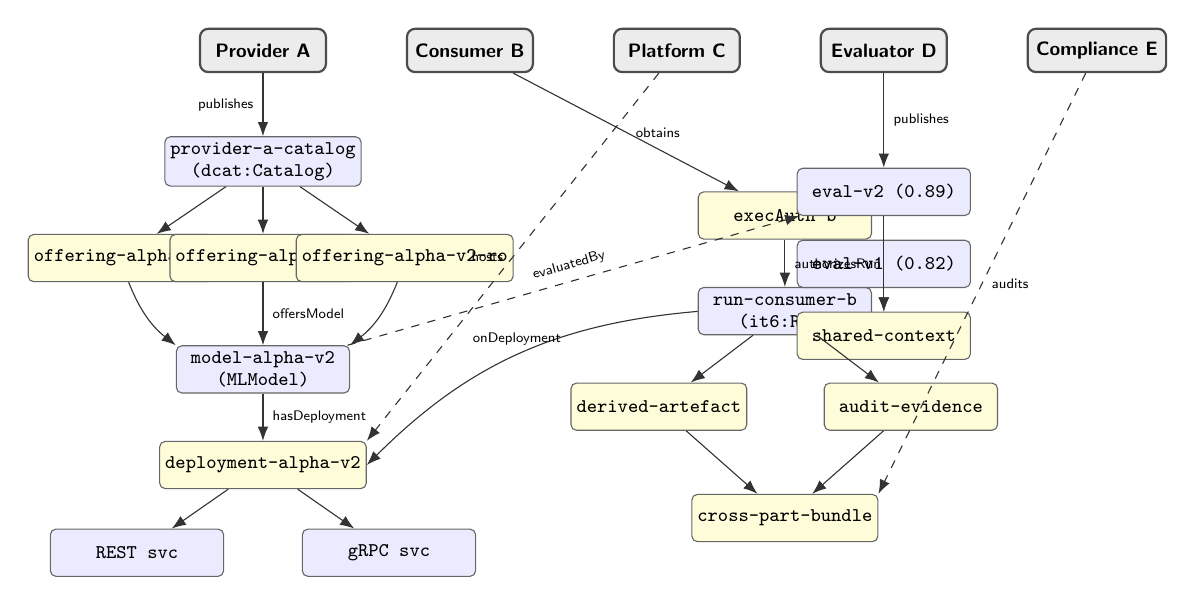
\begin{tikzpicture}[node distance=0.6cm and 0.8cm,
    instance/.style={rectangle, draw=black!60, fill=yellow!15, rounded corners=2pt,
      minimum width=2.2cm, minimum height=0.6cm, align=center, font=\ttfamily\scriptsize,
      inner sep=2pt},
    extinstance/.style={rectangle, draw=black!60, fill=blue!8, rounded corners=2pt,
      minimum width=2.2cm, minimum height=0.6cm, align=center, font=\ttfamily\scriptsize,
      inner sep=2pt},
    actorbox/.style={rectangle, draw=black!70, fill=gray!15, thick, rounded corners=3pt,
      minimum width=1.6cm, minimum height=0.55cm, align=center, font=\sffamily\scriptsize\bfseries,
      inner sep=3pt}]

  % Actors (top row, from left to right)
  \node[actorbox] (upm) {Provider~A};
  \node[actorbox, right=1.0cm of upm] (leg) {Consumer~B};
  \node[actorbox, right=1.0cm of leg] (inesdata) {Platform~C};
  \node[actorbox, right=1.0cm of inesdata] (csic) {Evaluator~D};
  \node[actorbox, right=1.0cm of csic] (gaia) {Compliance~E};

  % Publication layer
  \node[extinstance, below=0.8cm of upm] (catalog) {provider-a-catalog\\\scriptsize (dcat:Catalog)};
  \node[instance, below=0.6cm of catalog, xshift=-1.8cm] (off1) {offering-alpha-v2};
  \node[instance, below=0.6cm of catalog] (off2) {offering-alpha-v1};
  \node[instance, below=0.6cm of catalog, xshift=1.8cm] (off3) {offering-alpha-v2-ro};

  % Model and deployment
  \node[extinstance, below=0.8cm of off2] (model) {model-alpha-v2\\\scriptsize (MLModel)};
  \node[instance, below=0.6cm of model] (deploy) {deployment-alpha-v2};
  \node[extinstance, below=0.5cm of deploy, xshift=-1.6cm] (rest) {REST svc};
  \node[extinstance, below=0.5cm of deploy, xshift=1.6cm] (grpc) {gRPC svc};

  % Right side: authorization, run, derived, evidence
  \node[instance, below=1.5cm of leg, xshift=4cm] (auth) {execAuth-b};
  \node[extinstance, below=0.6cm of auth] (run) {run-consumer-b\\\scriptsize (it6:Run)};
  \node[instance, below=0.6cm of run, xshift=-1.6cm] (derived) {derived-artefact};
  \node[instance, below=0.6cm of run, xshift=1.6cm] (audit) {audit-evidence};

  % Bundle (bottom)
  \node[instance, below=0.8cm of derived, xshift=1.6cm] (bundle) {cross-part-bundle};

  % Evaluation (far right)
  \node[extinstance, below=1.2cm of csic] (eval2) {eval-v2 (0.89)};
  \node[extinstance, below=0.3cm of eval2] (eval1) {eval-v1 (0.82)};
  \node[instance, below=0.3cm of eval1] (ctx) {shared-context};

  % Arrows: publication
  \draw[objpropertyarrow] (upm) -- node[left, font=\tiny\sffamily] {publishes} (catalog);
  \draw[objpropertyarrow] (catalog) -- (off1);
  \draw[objpropertyarrow] (catalog) -- (off2);
  \draw[objpropertyarrow] (catalog) -- (off3);
  \draw[objpropertyarrow] (off2) -- node[right, font=\tiny\sffamily] {offersModel} (model);
  \draw[objpropertyarrow] (off1) to[bend right=15] (model.north west);
  \draw[objpropertyarrow] (off3) to[bend left=15] (model.north east);

  % Arrows: deployment and services
  \draw[objpropertyarrow] (model) -- node[right, font=\tiny\sffamily] {hasDeployment} (deploy);
  \draw[objpropertyarrow] (deploy) -- (rest);
  \draw[objpropertyarrow] (deploy) -- (grpc);

  % Arrows: authorization, run, derived, audit
  \draw[objpropertyarrow] (leg) -- node[right, font=\tiny\sffamily] {obtains} (auth);
  \draw[objpropertyarrow] (auth) -- node[right, font=\tiny\sffamily] {authorizesRun} (run);
  \draw[objpropertyarrow] (run) -- (derived);
  \draw[objpropertyarrow] (run) -- (audit);
  \draw[objpropertyarrow] (run) to[bend right=20] node[above, font=\tiny\sffamily] {onDeployment} (deploy.east);

  % Bundle aggregates
  \draw[objpropertyarrow] (derived) -- (bundle);
  \draw[objpropertyarrow] (audit) -- (bundle);

  % Evaluation side
  \draw[objpropertyarrow] (csic) -- node[right, font=\tiny\sffamily] {publishes} (eval2);
  \draw[objpropertyarrow] (eval2) -- (ctx);
  \draw[objpropertyarrow] (eval1) -- (ctx);
  \draw[objpropertyarrow, dashed] (model) -- node[above, font=\tiny\sffamily, sloped] {evaluatedBy} (eval2);

  % Governance audit
  \draw[objpropertyarrow, dashed] (gaia) -- node[right, font=\tiny\sffamily] {audits} (bundle.north east);
  \draw[objpropertyarrow, dashed] (inesdata) -- node[left, font=\tiny\sffamily] {hosts} (deploy.north east);

\end{tikzpicture}
\caption{Illustrative demonstrator instantiated over DAIMO with five anonymised participants. Grey rounded boxes on the top row are the five participants (one per \code{edc:ParticipantContext}); yellow-shaded instances are DAIMO-native (offerings, deployments, authorisations, derived artefacts, audit evidence, cross-participant bundle, shared evaluation context); light-blue instances are reused classes (catalog, model, services, runs, evaluations). Solid arrows denote direct properties; dashed arrows denote the participant's functional role over the instance below.}
\label{fig:scenario}
\end{figure*}

\subsection{Formal verification}\label{sec:eval-engineering}

Both reasoners agree. HermiT, invoked through \code{owlready2}, confirms that the union of the core, the alignments, and the example graph is logically consistent with no unsatisfiable classes; reasoning takes 0.72~s. OWL-RL materialisation (the \code{owlrl} library) derives 1\,171 additional triples on top of 817 initial ones (1\,988 in total) in 0.27~s, with no individuals typed as \code{owl:Nothing} and no unsatisfiable subclasses.

Logical consistency is necessary but not sufficient. An ontology may be consistent and still, for instance, infer that an \code{AuditEvidence} is a \code{prov:Activity}---a thing produced by activities, not an activity. That is why we added an entailment-verification check over the OWL-RL closure: for each native class, the script \code{reasoner\_check.py} enumerates every inferred superclass and tests it against a list of forbidden ones. The report covers the fourteen native classes (nine top-level plus five \code{ParticipantRole} subclasses) and raises no warning. This check is complementary to consistency: it catches alignment errors that a DL reasoner accepts because they are logically consistent yet semantically wrong.

The OOPS! scanner~\cite{oops14}, queried through its REST API on the union of the core and alignments, reports zero Critical pitfalls, zero Important ones, and two Minor ones: P13 (``inverse relationships not declared'') on 34 elements with no semantically meaningful inverse, and P04 (``isolated ontology elements'') on seven locally declared external classes. Both arise from the reuse-by-default discipline the profile applies.

The final layer of formal verification targets the alignment module itself. Seven \code{rdfs:subClassOf} and six \code{rdfs:subPropertyOf} declarations connect DAIMO to its five parent vocabularies (DCAT, MLDCAT-AP, ODRL, PROV-O, and FOAF). The entailment-verification check inspects the OWL-RL closure of each alignment and confirms that none produces a semantically incorrect superclass on any DAIMO-native class, raising zero warnings over the fourteen classes. We deliberately excluded three subproperty alignments toward PROV-O from the module for the same reason: each would have produced a forbidden typing under RDFS closure (§\ref{sec:axiomatic}).

\subsection{SHACL validation: structural, invariants, and negative test bench}\label{sec:eval-invariants}

DAIMO layers three SHACL \emph{shape} families, each answering a different validation question. Structural shapes ask whether every DAIMO-native instance carries the mandatory properties of its class. Conformance shapes ask whether reused external classes satisfy the additional obligations that the profile imposes on them. SPARQL invariants ask whether relations across several classes remain coherent. Together, the three families move validation from syntactic to semantic: from ``is this instance well-formed?'' to ``is this graph internally consistent?''.

The nine structural shapes impose minimum completeness per DAIMO class, and the 225-triple positive graph satisfies \code{conforms=True}. The three conformance shapes add operational obligations on reused classes: \code{OfferInDAIMOShape} requires every \code{odrl:Offer} used in DAIMO to declare \code{odrl:assigner} and \code{odrl:target} (at policy level or per permission, through \code{sh:or}); \code{MachineLearningModelInDAIMOShape} requires an ODRL policy, title, and identifier on \code{it6:MachineLearningModel}; \code{RunInDAIMOShape} requires flow, algorithm, associated agent, and timestamp on \code{it6:Run}. Additionally, \code{sh:in} restricts \code{daimo:authMethod} values to a closed vocabulary of nine tokens (\code{none}, \code{api-key}, \code{basic}, \code{bearer}, \code{oauth2-bearer}, \code{oauth2-client-credentials}, \code{mtls}, \code{jwt}, \code{dataspace-token}), and \code{sh:pattern} restricts \code{daimo:protocol} to a pattern accepting the usual evaluation-protocol names (\code{holdout}, \code{stratified-holdout}, \code{leave-one-out}, \code{temporal-split}, \code{<n>-fold-cv}, \code{stratified-<n>-fold-cv}, \code{bootstrap-<n>}).

Above this structural stratum sit the six SHACL-SPARQL cross-class invariants, encoded through \code{sh:SPARQLConstraint}. They are the differentiator against a purely descriptive profile. INV-1 guarantees consistency of the derivation-authorisation chain: every \code{DerivedArtifact} must carry a \code{daimo:underAuthorization} property whose authorisation covers precisely the execution the artefact is derived from. INV-2 forces the agent associated with an execution through \code{prov:wasAssociatedWith} to also appear as \code{daimo:grantedTo} on one of the authorisations covering that execution, making explicit that the PROV-registered actor and the ODRL-authorised beneficiary must be the same entity. INV-3 checks data-plane coherence: the \code{dcat:DataService} exposed by a \code{ModelDeployment} must serve exactly the model the deployment declares, ruling out an endpoint that advertises one model and serves another. INV-4 requires \code{daimo:expiresAt} of every \code{ExecutionAuthorization} to be strictly later than \code{prov:startedAtTime} of every execution the authorisation covers, reflecting that an authorisation cannot justify executions that started after it lapsed. INV-5 requires the model referenced by \code{daimo:offersModel} in an \code{AIAssetOffering} to appear as \code{odrl:target} of the attached policy, at policy level or in one of its permissions; if the policy does not govern the registered model, the governance chain is broken even if both resources exist. INV-6 closes the same triangle on the provider side: \code{daimo:offeredBy} of every offering must equal \code{odrl:assigner} of its policy, preventing inconsistencies between the catalog-record attribution and the ODRL offer's declared authorship. The positive graph conforms to all six invariants without warnings.

Listing~\ref{lst:inv5} shows the concrete encoding of INV-5 as \code{sh:SPARQLConstraint}, illustrating the \code{FILTER NOT EXISTS} pattern that captures the disjunction between policy-level and per-permission targets.

\begin{lstlisting}[label=lst:inv5,caption={INV-5 encoded as a \code{sh:SPARQLConstraint}.}]
daimo:OfferingPolicyTargetInvariant a sh:NodeShape ;
    sh:targetClass daimo:AIAssetOffering ;
    sh:sparql [
        a sh:SPARQLConstraint ;
        sh:message "INV-5 violation: offering's offersModel does not
                    appear as odrl:target of the attached policy."@en ;
        sh:prefixes daimo:_invariantPrefixes ;
        sh:select """
            SELECT $this ?model ?policy WHERE {
                $this daimo:offersModel ?model ;
                      daimo:hasOfferPolicy ?policy .
                FILTER NOT EXISTS { ?policy odrl:target ?model }
                FILTER NOT EXISTS { ?policy odrl:permission/odrl:target ?model }
            }
        """ ;
    ] .
\end{lstlisting}

Shapes that conform on the positive graph are necessary but not sufficient to show that constraints are semantically discriminating. A trivially satisfiable constraint on any graph would pass positive validation without yielding real guarantees. For this reason DAIMO ships a companion graph \code{tests/negative-examples.ttl} (118 triples) that encodes six deliberately invalid cases (\code{bad:INV1-artifact}, \code{bad:INV2-run}, \code{bad:INV3-deployment}, \code{bad:INV4-auth}, \code{bad:INV5-offering}, and \code{bad:INV6-offering}), each crafted to violate exactly one invariant. The \code{tests/negative\_test.py} script loads the ontology, the shapes, and the negative graph, runs SHACL, and verifies two conditions: global validation fails, and every expected focus node appears in the report with the specific invariant's message. All six invariants fire correctly on their designated violation. This evidence complements positive validation and is what allows us to claim, with grounding, that the invariants capture real business rules.

\subsection{Competency questions}\label{sec:eval-cqs}

The twenty-three competency questions are expressed as SPARQL queries (\code{queries/queries.md}) and run over the OWL-RL materialised closure of the positive graph. Table~\ref{tab:cqs} summarises coverage by category, observed row counts, and queries requiring explicit reasoning; the full set of queries appears in Appendix~\ref{app:sparql}. All twenty-three return at least one row, which confirms that the demonstration graph contains the information needed to answer every question with the primitives DAIMO declares.

\begin{table*}[t]
\small\sf\centering
\caption{Coverage of the 23 competency questions. Each CQ returns the indicated row count over the positive graph under OWL-RL closure. Boldface marks queries that require explicit reasoning beyond plain SPARQL.\label{tab:cqs}}
\begin{tabular}{@{}p{3.3cm}p{2.6cm}p{0.8cm}p{6.3cm}@{}}
\toprule
\textbf{Category} & \textbf{Queries (rows)} & \textbf{N} & \textbf{Inference required} \\
\midrule
Registration and publication (R) & R1(3) R2(1) R3(1) R4(2) R5(2) & 5 & \textbf{R2} (\code{subPropertyOf} chain), \textbf{R5} (\code{subClassOf} path) \\
Discovery and selection (D) & D1(3) D2(2) D3(4) D4(1) & 4 & \textbf{D1} (task subtype), \textbf{D2} (policy matching) \\
Execution and auditability (E) & E1(4) E2(1) E3(2) E4(1) E5(1) & 5 & \textbf{E1} (\code{offersModel}~$\sqsubseteq$~\code{foaf:primaryTopic}), \textbf{E2} (agreement-run union) \\
Evaluation and reproducibility (V) & V1(1) V2(1) V3(2) V4(1) V5(4) & 5 & \textbf{V2}, \textbf{V3} (aggregation) \\
Governance bridge (G) & G1(1) G2(2) G3(1) G4(1) & 4 & \textbf{G3} (\code{subClassOf} reasoning), \textbf{G4} (\code{GROUP\_CONCAT} aggregation) \\
\bottomrule
\end{tabular}
\end{table*}

Two observations deserve emphasis. CQ-R2 and CQ-E1 depend on the \code{subPropertyOf} relation between \code{daimo:offersModel} and \code{foaf:primaryTopic} and return no rows on a plain SPARQL engine without reasoning. The dependency is documented rather than defective: aligning \code{offersModel} under \code{foaf:primaryTopic} makes offerings discoverable through the standard DCAT property, a benefit that materialises only under inference. A consumer who must run those queries on a plain endpoint can materialise the closure beforehand or rewrite the queries to enumerate both properties. The second observation is that CQ-G2 returns two rows, one per endpoint of the multi-protocol REST and gRPC deployment. This confirms that modelling several services per deployment is a legitimate, directly SPARQL-observable pattern.

Two fragments illustrate the pattern. Listing~\ref{lst:cq-g3} shows CQ-G3 (``which authorisation authorised a specific run, and which ODRL agreement backs it?''): the query traverses the \code{daimo:authorizedBy} inverse from an \code{it6:Run} to an \code{ExecutionAuthorization}, then lifts the agreement's assigner and assignee. Listing~\ref{lst:cq-v3} shows CQ-V3 (``ranking of models under the same \code{SharedEvaluationContext} and metric''): the query joins evaluations against a fixed context, orders by metric value, and binds the model and the run that produced each evaluation. Both queries run over the OWL-RL-materialised closure of the demonstrator; the full twenty-three SPARQL queries are published in \code{queries/queries.md} for inspection.

\begin{lstlisting}[label=lst:cq-g3,caption={CQ-G3: authorisation and agreement for a specific run.}]
SELECT ?auth ?assigner ?assignee WHERE {
    ?run a it6:Run ;
         daimo:authorizedBy ?auth .
    ?auth a daimo:ExecutionAuthorization ;
          odrl:assigner ?assigner ;
          odrl:assignee ?assignee .
    FILTER (?run = <https://example.org/daimo-scenario/run-consumer-b>)
}
\end{lstlisting}

\begin{lstlisting}[label=lst:cq-v3,caption={CQ-V3: ranking of models under a shared evaluation context.}]
SELECT ?model ?metric ?value WHERE {
    ?eval a it6:Evaluation ;
          daimo:hasEvaluationContext ?ctx ;
          it6:hasMeasure ?m .
    ?m it6:metricType ?metric ;
       it6:metricValue ?value .
    ?run it6:hasEvaluation ?eval ;
         daimo:onDeployment/daimo:deploysModel ?model .
    FILTER (?ctx = <https://example.org/daimo-scenario/eval-context>)
} ORDER BY DESC(?value)
\end{lstlisting}


% =====================================================================
\section{Discussion}\label{sec:discussion}

DAIMO connects publication, policy, execution, provenance, and evaluation in a single profile. That articulation sustains governed AI-model exchange across organisational boundaries, and it distinguishes DAIMO both from recent domain ontologies (RePlanIT~\cite{kurteva}, GloSIS~\cite{palma}, Woods et al.~\cite{woods}) and from earlier machine-learning lifecycle ontologies. With the former, DAIMO shares an engineering ethos of reuse, executable implementation, and CQ-based evaluation, but applies it to the catalog-dataspace bridge. With the latter, DAIMO shares the application domain but adds the governance layer they do not address. Three design features set the artefact apart. First, entailment verification over the OWL-RL closure complements consistency reasoning: it enumerates inferred superclasses of each native class and detects semantically wrong alignments a DL reasoner accepts without contradiction. Second, cross-class SHACL-SPARQL invariants are paired with a negative test bench; every invariant fires on a case built to violate it, not only on the positive graph. Third, reuse is axiomatic, not nominal: seven explicit \code{rdfs:subClassOf} and six \code{rdfs:subPropertyOf} declarations, plus three deliberately undeclared subproperties whose adoption would have introduced unintended typings.

Three lines of argument bound the limitations. The first concerns \emph{semantic depth}. \code{IOContract} captures I/O format and authentication method (restricted by \code{sh:in} to a closed vocabulary) but not fine-grained semantic compatibility between model and consumer schemas, which is delegated to \code{it6:Flow} as Kipoi~\cite{kipoi} and TFX~\cite{tfx} do for preprocessing and pipelines. \code{SharedEvaluationContext} reifies task-dataset-version-protocol-seed for single-metric comparisons; heterogeneous benchmarking protocols and composite metric sets remain open. The role model folds role type (\code{ModelProvider}) into role assignment (the agent-role-context-scope tuple), which OntoClean recommends splitting. MLDCAT-AP folds them the same way in \code{hasRegisteredUser}, which places fine-grained contextualisation in the future-refinement horizon, not at the level of a present design error.

The second line concerns the \emph{integration commitments} and their effects on consumers who combine DAIMO with adjacent vocabularies. Property \code{daimo:records} declares \code{rdfs:range~prov:Activity}: under RDFS reasoning, MLDCAT-AP evaluations grouped inside a \code{CrossParticipantProvenanceRecord} are inferred as PROV activities even though MLDCAT-AP does not declare that subsumption. The effect is harmless for audit queries, but a consumer combining DAIMO, MLDCAT-AP, and PROV-O may see surprising typings on \code{it6:Evaluation}. Relatedly, DAIMO is not anchored to an upper ontology (BFO, GFO, DOLCE, UFO). The absence is intentional, because an integration profile is not a reference ontology. A coherent future step would be to accommodate the taxonomy to one of these upper ontologies without giving up direct reuse of the domain vocabularies that motivate DAIMO.

The third line concerns \emph{reproducibility conditions and external validation}. Reported numerical results depend on a specific reasoning profile: \code{inference=rdfs} mode in pyshacl, necessary for implied subproperties to materialise before the conformance shapes are evaluated, and the OWL-RL closure materialised before the competency queries. This dependency is documented but is a condition a consumer must know to reproduce exact results. Expert-based validation is not part of the evidence reported here; a qualitative study with three practitioner profiles (an EDC or INESData engineer, an MLDCAT-AP/SEMIC maintainer, and an MLOps practitioner) is the next phase of work. \TODO{Run the expert study: recruitment, semi-structured interview protocol, qualitative analysis, and publication of results.}

Adoption and envisaged integration paths are concrete even though a deployed pilot is not part of the present evidence. On the AI-asset side, DAIMO is designed to co-evolve with the SEMIC MLDCAT-AP dossier: it reuses the 3.0.0 vocabulary directly and adds no classes that overlap the MLDCAT-AP scope, which keeps a MLDCAT-AP-native consumer compatible without translation. On the dataspace side, the natural integration host is Eclipse Dataspace Components: DAIMO references \code{edc:ParticipantContext} explicitly to anchor aggregated provenance, and its ODRL agreements are standard \code{odrl:Agreement} instances that an EDC connector already produces at the end of a DSP negotiation. On the governance side, DAIMO's \code{AuditEvidence} class is structured to carry the integrity records that a Gaia-X Trust Framework inspection, or an AI Act Annex IV traceability audit, would request: checksum, signer, timestamp, and linkage to a cross-participant bundle. We envisage three concrete validation paths for adoption: instantiation over a public MLDCAT-AP catalog extract (to verify the reuse claims under real metadata), co-deployment with an EDC connector on a federated pilot (to witness the DSP-to-\code{ExecutionAuthorization} chain end-to-end), and mapping of a high-risk AI Act use case against the six SHACL-SPARQL invariants (to assess operational fit). None of these has been executed yet; they define the short-term adoption roadmap rather than the present claims.

The relation between DAIMO and MLDCAT-AP deserves explicit delimitation. The model itself is reused directly through \code{it6:MachineLearningModel}. DAIMO's contribution concentrates on the catalog-dataspace bridge: the four competency questions of the governance category exercise exclusively DAIMO-native classes and cannot be answered with MLDCAT-AP alone, because they require \code{AIAssetOffering} (CQ-G1), \code{ModelDeployment} (CQ-G2), \code{ExecutionAuthorization} (CQ-G3), and \code{CrossParticipantProvenanceRecord} (CQ-G4). The two profiles are complementary.

Looking beyond the present artefact, DAIMO illustrates a pattern that is likely to recur wherever autonomous participants need to exchange high-value, policy-bound resources. The pattern has three recurring elements: an offering record reified above the resource itself, an authorisation reified above the permission, and a provenance bundle that crosses administrative contexts. Genomic datasets, clinical decision-support tools, digital twins, and industrial models all present analogous publication-invocation-auditing chains. DAIMO is AI-specific in what it reuses (MLDCAT-AP) but domain-agnostic in the constructs it adds, and we hope the constructs will serve as a starting point for sibling profiles in adjacent domains.

\medskip
\noindent\textbf{Availability and FAIR compliance.}\label{sec:avail}
DAIMO is distributed as a public package under CC-BY~4.0 (ontology and documentation) and Apache~2.0 (validation scripts). The artefact is \emph{findable} through the persistent \code{w3id.org/pionera/daimo} namespace with per-version IRIs and Dublin Core metadata; \emph{accessible} through content negotiation across Turtle, RDF/XML, JSON-LD, and N-Triples; \emph{interoperable} through exclusive reuse of W3C-standard vocabularies and OWL~2~DL profile; and \emph{reusable} through SKOS definitions and examples per term, SemVer versioning (with a deprecation policy based on \code{owl:deprecated} and \code{skos:closeMatch}), and SHACL shapes that act as a data contract. Appendix~\ref{app:avail} lists the deliverable items and their locations, and the full release procedure is documented in \code{DEPLOYMENT.md} so that any future maintainer can run it without implicit knowledge.

% =====================================================================
\section{Conclusions}\label{sec:conclusion}

DAIMO's delta over the reused vocabularies is the governance bridge between the AI catalog and the dataspace: offering, authorisation, deployment, derived artefact, and cross-participant provenance. The four governance-category competency questions witness the gap concretely; they cannot be answered with any of the reused vocabularies alone. Entailment verification, a negative SHACL-SPARQL test bench, and the reproducible demonstrator provide three complementary mechanisms of evidence. Future work follows from the bounded limitations: external expert validation, instantiation over a public MLDCAT-AP catalog, refinement of \code{IOContract} toward schema compatibility, role-type/role-assignment split following OntoClean, and extension of \code{SharedEvaluationContext} to heterogeneous benchmarking protocols. The package is published under CC-BY~4.0 (ontology) and Apache~2.0 (scripts) and is ready to be adopted, extended, or challenged by the community.

% =====================================================================
\begin{thebibliography}{40}

\bibitem{franklin05} Franklin, M., Halevy, A. and Maier, D. (2005) From Databases to Dataspaces: A New Abstraction for Information Management. \emph{SIGMOD Record}, 34(4):27--33.

\bibitem{dcat2} Albertoni, A. et al. (2020) \emph{Data Catalog Vocabulary (DCAT) --- Version 2}. W3C Recommendation.

\bibitem{provo} Lebo, P., Sahoo, S. and McGuinness, D. (eds.) (2013) \emph{PROV-O: The PROV Ontology}. W3C Recommendation.

\bibitem{odrl22} Iannella, R., Guth, S. and Steyskal, R. (eds.) (2018) \emph{ODRL Information Model 2.2}. W3C Recommendation.

\bibitem{shacl} Knublauch, H. and Kontokostas, D. (eds.) (2017) \emph{Shapes Constraint Language (SHACL)}. W3C Recommendation.

\bibitem{mitchell19} Mitchell, M. et al. (2019) Model Cards for Model Reporting. \emph{Proceedings of the Conference on Fairness, Accountability, and Transparency}.

\bibitem{arnold19} Arnold, M. et al. (2019) FactSheets: Increasing Trust in AI Services through Supplier's Declarations of Conformity. \emph{IBM Research Report}.

\bibitem{werbrouck24} Werbrouck, J. et al. (2024) ConSolid: A federated ecosystem for heterogeneous multi-stakeholder projects. \emph{Semantic Web}, 15:429--460.

\bibitem{kurteva} Kurteva, A. et al. (in press) RePlanIT Ontology for Digital Product Passports of ICT: Laptops and Data Servers. \emph{Semantic Web}.

\bibitem{palma} Palma, R. et al. (in press) GloSIS: The Global Soil Information System Web Ontology. \emph{Semantic Web}.

\bibitem{woods} Woods, C. et al. (in press) An ontology for maintenance activities and its application to data quality. \emph{Semantic Web}.

\bibitem{penteado23} Penteado, B.E., Maldonado, J.C. and Isotani, S. (2023) Methodologies for publishing linked open government data on the Web. \emph{Semantic Web}, 14:585--610.

\bibitem{bareedu24} Bareedu, Y.S. et al. (2024) Deriving semantic validation rules from industrial standards: An OPC UA study. \emph{Semantic Web}, 15:517--554.

\bibitem{ferranti} Ferranti, N. et al. (in press) Formalizing and Validating Wikidata's Property Constraints using SHACL and SPARQL. \emph{Semantic Web}.

\bibitem{pandit-esteves} Pandit, H.J. and Esteves, B. (in press) Enhancing Data Use Ontology (DUO) for Health-Data Sharing by Extending it with ODRL and DPV. \emph{Semantic Web}.

\bibitem{robaldo} Robaldo, L. and Batsakis, S. (in press) On the interplay between validation and inference in SHACL. \emph{Semantic Web}.

\bibitem{otto19} Otto, B. et al. (2019) Reference architecture model for international data spaces. \emph{International Journal of Information Management}, 45:182--199.

\bibitem{cappiello22} Cappiello, C., Gal, A., Jarke, M., Rehof, J. and Yang, Y. (2022) Data spaces: Design, deployment, and future directions. \emph{ACM Computing Surveys}, 55(2):Article~46.

\bibitem{gebru21} Gebru, T. et al. (2021) Datasheets for datasets. \emph{Communications of the ACM}, 64(12):86--92.

\bibitem{kipoi} Avsec, Z. et al. (2019) The Kipoi repository accelerates community exchange and reuse of predictive models for genomics. \emph{Nature Biotechnology}, 37.

\bibitem{tfx} Baylor, D. et al. (2017) TFX: A TensorFlow-based production-scale machine learning platform. \emph{KDD}.

\bibitem{expo} Soldatova, L.N. and King, R.D. (2006) An ontology of scientific experiments. \emph{Journal of the Royal Society Interface}, 3(11).

\bibitem{mls} Correa Publio, G. et al. (2018) ML-Schema: Exposing the semantics of machine learning with schemas and ontologies.

\bibitem{mex} Keet, C.M., Fernández, J.D. and Panov, P. (2016) MEX vocabulary: A lightweight interchange format for machine learning experiments. \emph{ISWC}.

\bibitem{ontodm} Panov, P., Dzeroski, S. and Soldatova, L.N. (2008) OntoDM: An ontology of data mining. \emph{ICDMW}.

\bibitem{dmop} Keet, C.M. et al. (2015) The data mining optimization ontology. \emph{Web Semantics}, 32.

\bibitem{souza19} Souza, R. et al. (2019) Provenance data in the machine learning lifecycle in computational science and engineering. \emph{WORKS}.

\bibitem{schmidt21} Schmidt, M. et al. (2021) FAIRness along the machine learning lifecycle using Dataverse in combination with MLflow. \emph{ICDE Workshops}.

\bibitem{lot22} Poveda-Villalón, M., Fernández-Izquierdo, A., Fernández-López, M. and García-Castro, R. (2022) LOT: An industrial oriented ontology engineering framework. \emph{Engineering Applications of Artificial Intelligence}, 111:104755.

\bibitem{oops14} Poveda-Villalón, M., Gómez-Pérez, A. and Suárez-Figueroa, M.C. (2014) OOPS! (OntOlogy Pitfall Scanner!). \emph{International Journal on Semantic Web and Information Systems}, 10(2):7--34.

\bibitem{mldcatap} SEMIC (2025) \emph{MLDCAT-AP 3.0.0: Machine Learning Data Catalogue Application Profile}. European Commission.

\bibitem{dsp} International Data Spaces Association (2024) \emph{Dataspace Protocol (DSP)}. W3C Community Draft.

\bibitem{edc} Eclipse Foundation. \emph{Eclipse Dataspace Components (EDC)}, control-plane documentation.

\bibitem{widoco} Garijo, D. (2017) WIDOCO: A Wizard for Documenting Ontologies. \emph{ISWC}.

\bibitem{aiact} European Union (2024) \emph{Regulation (EU) 2024/1689 laying down harmonised rules on artificial intelligence (AI Act)}. Official Journal of the European Union.

\end{thebibliography}

% =====================================================================
\appendix

\section{Artefact availability}\label{app:avail}

\begin{table}[h]
\small\sf\centering
\caption{Deliverable items of the DAIMO public package and their locations.\label{tab:avail}}
\begin{tabular}{@{}p{4cm}p{11cm}@{}}
\toprule
\textbf{Item} & \textbf{Location} \\
\midrule
Persistent namespace & \url{https://w3id.org/pionera/daimo} --- \TODO{Merge the PR on \texttt{perma-id/w3id.org} so that the namespace resolves via content negotiation.} \\
Versioned modules & Three independent ontologies (core, shapes, alignments) under \url{https://w3id.org/pionera/daimo/} with explicit \code{owl:versionIRI} and \code{owl:priorVersion} \\
Public repository & \TODO{Create public GitHub repository \texttt{pionera/daimo} by running \texttt{DEPLOYMENT.md} and include the final URL here.} \\
Versioned archival (DOI) & \TODO{Archive the first release in Zenodo and include the resulting DOI here.} \\
Serialisations & Turtle, RDF/XML, JSON-LD, N-Triples (pre-generated by WIDOCO) \\
HTML documentation & WIDOCO 1.4.25 with WebVOWL; content negotiation via \code{.htaccess} under \code{w3id-redirect/} \\
Human-readable reference & \code{ONTOLOGY-REFERENCE.md} (class by class, with \code{skos:definition}, \code{skos:example}, identity criteria, OntoClean tags) and \code{VALIDATION-MATRIX.md} \\
Release metadata & \code{CITATION.cff}, \code{.zenodo.json}, \code{CHANGELOG.md} \\
Validation package & \code{validate.py}, \code{reasoner\_check.py}, \code{oops\_check.py}, \code{tests/negative\_test.py} \\
Maintenance governance & \code{CONTRIBUTING.md} (LOT Phase 4: issue triage, pull requests, SemVer, deprecation policy) \\
\bottomrule
\end{tabular}
\end{table}

The reproducibility workflow does not require prior deployment of the persistent URL. Any user with Python~3.12 and the declared dependencies (\code{rdflib}, \code{pyshacl}, \code{owlrl}, \code{owlready2}) can run the four scripts locally and reproduce every report in \code{reports/}. The persistent URL and the DOI are additional FAIR requirements that complement but do not condition reproducibility.

\section{Competency questions}\label{app:cqs}

\subsection*{R --- Registration and publication (5)}
\begin{enumerate}[label=\arabic*., leftmargin=*]
\item \cq{CQ-R1}: Which AI models has a given provider published as governed catalog assets?
\item \cq{CQ-R2}: For a given model, which catalog offering registered it, by which publisher, and when? (requires \code{subPropertyOf} chain)
\item \cq{CQ-R3}: Licence and usage policy of a model.
\item \cq{CQ-R4}: I/O contract for the invocation interface of a published model.
\item \cq{CQ-R5}: For each offering, what concrete \code{ParticipantRole} subclass does the providing agent hold? (requires \code{subClassOf+})
\end{enumerate}

\subsection*{D --- Discovery and selection (4)}
\begin{enumerate}[label=\arabic*., leftmargin=*]
\item \cq{CQ-D1}: Which models solve a given task in a given application domain?
\item \cq{CQ-D2}: Which of those models are usable under a non-commercial policy pattern?
\item \cq{CQ-D3}: Which models expose a service endpoint, and what authentication method does each require?
\item \cq{CQ-D4}: Models reaching a minimum metric threshold under a shared evaluation context.
\end{enumerate}

\subsection*{E --- Execution and auditability (5)}
\begin{enumerate}[label=\arabic*., leftmargin=*]
\item \cq{CQ-E1}: For a given catalog offering, what service endpoint, authentication, and I/O contract apply to invoking the underlying model? (requires entailment)
\item \cq{CQ-E2}: For a given model deployment, which runs have been executed, by which agents, and under which execution authorisation?
\item \cq{CQ-E3}: Implementation, algorithm, flow, and compute infrastructure used in a run.
\item \cq{CQ-E4}: Audit evidence (hash, signer, timestamp) supporting a given run.
\item \cq{CQ-E5}: Derived artefacts produced by a run, and under which authorisation.
\end{enumerate}

\subsection*{V --- Evaluation and reproducibility (5)}
\begin{enumerate}[label=\arabic*., leftmargin=*]
\item \cq{CQ-V1}: Shared evaluation context of a given evaluation.
\item \cq{CQ-V2}: Under a shared evaluation context, highest-scoring model for a metric.
\item \cq{CQ-V3}: Ranking of models under the same evaluation context and metric.
\item \cq{CQ-V4}: For a given model, which benchmark suites has it been evaluated on?
\item \cq{CQ-V5}: Reproducibility artefacts backing an evaluation.
\end{enumerate}

\subsection*{G --- Governance bridge (4, DAIMO-native)}
\begin{enumerate}[label=\arabic*., leftmargin=*]
\item \cq{CQ-G1}: Offerings that include a given model.
\item \cq{CQ-G2}: Deployments serving a model, with infrastructure and I/O contract.
\item \cq{CQ-G3}: Authorisation (and agreement) that authorised a specific run.
\item \cq{CQ-G4}: Full provenance bundle for a derived artefact across participant contexts.
\end{enumerate}

\section{SHACL shapes}\label{app:shapes}

The DAIMO SHACL layer contains nine structural nodal shapes, three conformance shapes over reused classes, and six cross-class SHACL-SPARQL invariants. The module \code{shapes/daimo-shapes.ttl} is itself declared as an independent \code{owl:Ontology} with its own \code{owl:versionIRI} under \url{https://w3id.org/pionera/daimo/shapes/}.

\begin{itemize}[leftmargin=*]
\item \textbf{Completeness shapes (9)}: \code{AIAssetOfferingShape}, \code{ParticipantRoleShape}, \code{ModelDeploymentShape}, \code{IOContractShape}, \code{ExecutionAuthorizationShape}, \code{DerivedArtifactShape}, \code{SharedEvaluationContextShape}, \code{AuditEvidenceShape}, \code{CrossParticipantProvenanceRecordShape}.
\item \textbf{Conformance shapes over reused classes (3)}: \code{OfferInDAIMOShape} requires \code{odrl:assigner} and \code{odrl:target} on every \code{odrl:Offer}; \code{MachineLearningModelInDAIMOShape} requires policy, title, and identifier on \code{it6:MachineLearningModel}; \code{RunInDAIMOShape} requires flow, algorithm, associated agent, and timestamp on \code{it6:Run}.
\item \textbf{Cross-class invariants (6)}: \code{DerivationAuthorizationInvariant} (INV-1), \code{RunAgentAuthorizationInvariant} (INV-2), \code{DeploymentServiceInvariant} (INV-3), \code{AuthorizationTemporalInvariant} (INV-4), \code{OfferingPolicyTargetInvariant} (INV-5), and \code{OfferingAssignerInvariant} (INV-6); all encoded as \code{sh:SPARQLConstraint}.
\end{itemize}

\section{SPARQL queries}\label{app:sparql}

The twenty-three SPARQL queries for the competency questions of Appendix~\ref{app:cqs} are published in \code{queries/queries.md}. The validator runs each query over the OWL-RL closure of the ontology-plus-example graph and verifies that each returns at least one row. Exact counts appear in Table~\ref{tab:cqs}. CQ-G2 returns two rows (one per endpoint of the REST/gRPC multi-protocol deployment), confirming that modelling multiple services per deployment is a legitimate pattern directly observable from SPARQL.

\section{Glossary of abbreviations}\label{app:glossary}

\begin{table}[h]
\small\sf\centering
\caption{Abbreviations used in this article.\label{tab:glossary}}
\begin{tabular}{@{}p{2.2cm}p{5.3cm}@{}}
\toprule
\textbf{Abbrev.} & \textbf{Expansion} \\
\midrule
AI Act & Regulation (EU) 2024/1689 on artificial intelligence \\
BFO & Basic Formal Ontology \\
CQ & Competency Question \\
DAIMO & Data-space AI Model Ontology \\
DCAT & Data Catalog Vocabulary \\
DCAT-AP & DCAT Application Profile \\
DL & Description Logic \\
DOI & Digital Object Identifier \\
DPV & Data Privacy Vocabulary \\
DSP & Dataspace Protocol \\
EDC & Eclipse Dataspace Components \\
FAIR & Findable, Accessible, Interoperable, Reusable \\
FOAF & Friend Of A Friend vocabulary \\
GFO & General Formal Ontology \\
I/O & Input / Output \\
LOT & Linked Open Terms methodology \\
MLDCAT-AP & Machine Learning Data Catalogue Application Profile \\
OOPS! & OntOlogy Pitfall Scanner \\
ODRL & Open Digital Rights Language \\
OWL & Web Ontology Language \\
OWL-RL & OWL 2 RL profile / rule-based reasoning \\
PROV-O & PROV Ontology \\
RDF & Resource Description Framework \\
RDFS & RDF Schema \\
REST & Representational State Transfer \\
SHACL & Shapes Constraint Language \\
SKOS & Simple Knowledge Organization System \\
SPARQL & SPARQL Protocol and RDF Query Language \\
SPDX & Software Package Data Exchange \\
SWJ & Semantic Web Journal \\
TTL & Turtle (RDF serialisation) \\
UFO & Unified Foundational Ontology \\
WIDOCO & Wizard for Documenting Ontologies \\
\bottomrule
\end{tabular}
\end{table}

\section{URI conventions}\label{app:uris}

DAIMO uses the canonical namespace \url{https://w3id.org/pionera/daimo}, with term identifiers of the form \code{https://w3id.org/pionera/daimo\#<Term>} and versioned IRIs under \code{https://w3id.org/pionera/daimo/<version>}, linked to each other through \code{owl:priorVersion}. The satellite modules are independent ontologies with their own versioned IRIs: the SHACL layer under \url{https://w3id.org/pionera/daimo/shapes/} and the alignment module under \url{https://w3id.org/pionera/daimo/align} (the latter declaring \code{owl:imports} on the base ontology). The example graph uses the local namespace \code{https://example.org/daimo-scenario/}, clearly separated from the canonical space to avoid confusion between demonstration identifiers and ontology terms. Content negotiation resolves the same identifier to HTML, Turtle, RDF/XML, JSON-LD, or N-Triples depending on the \code{Accept} header; the corresponding \code{.htaccess} configuration is prepared under \code{w3id-redirect/.htaccess} pending integration in \code{perma-id/w3id.org}.

\end{document}
